\section*{Answer 1}
\label{answer-1}

\begin{figure}[ht] % SS of TM
  \centering
  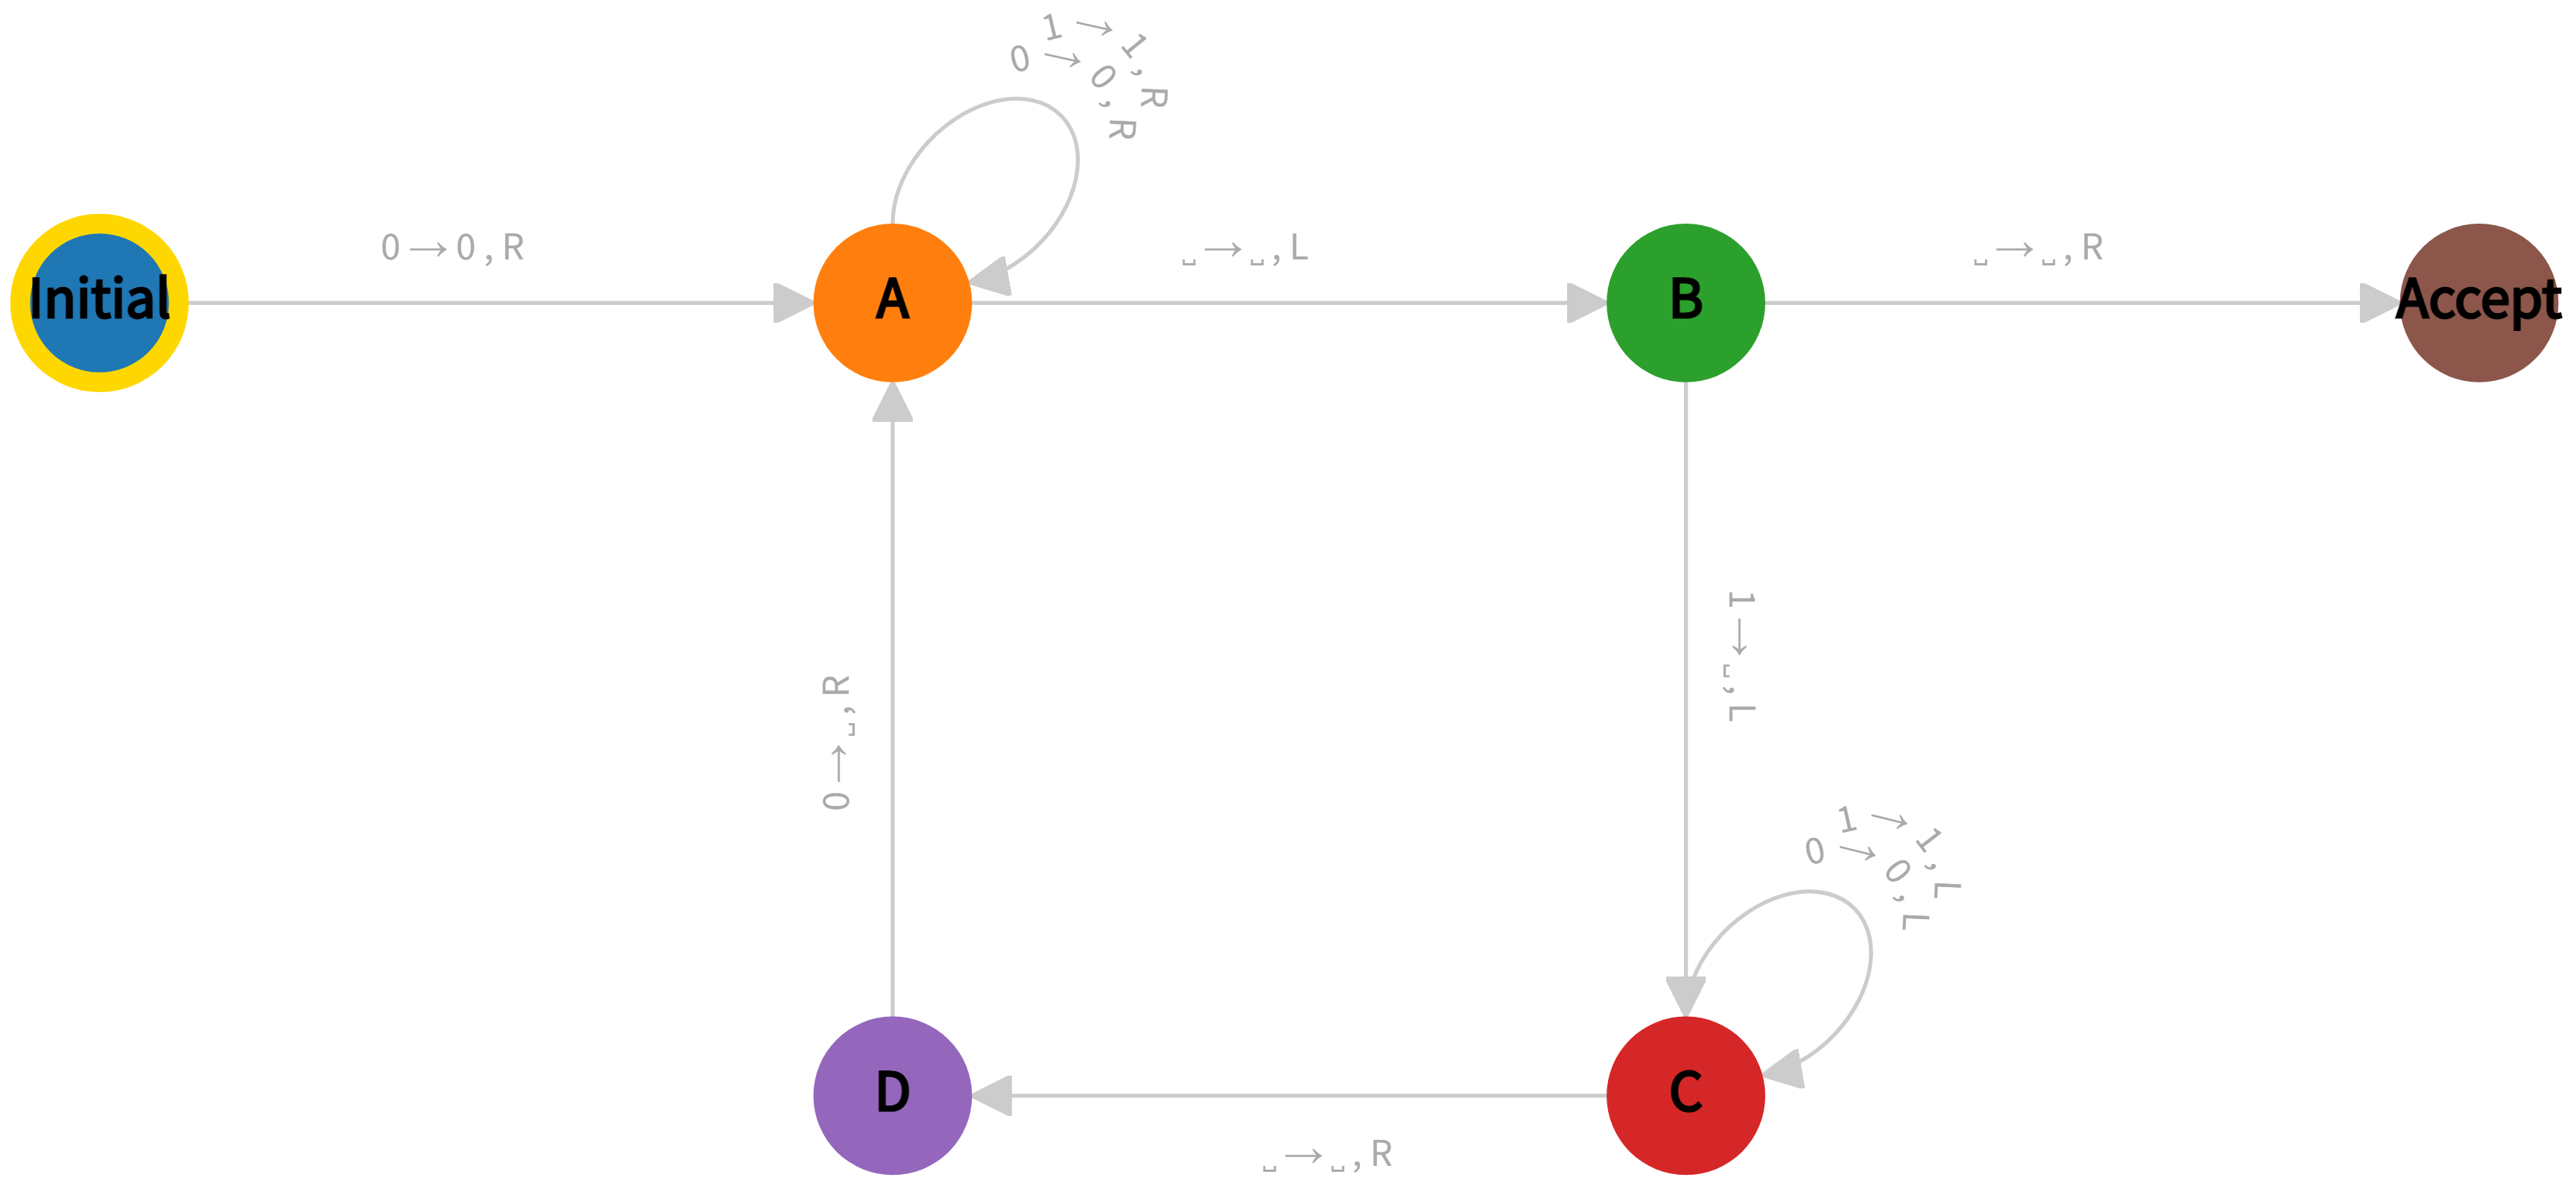
\includegraphics[width=\linewidth]{answers/img/q1-machine.png}
  \caption{\textit{Screenshot of the Turing Machine designed for Q1}}
  \label{fig:q1-machine}
\end{figure}

\begin{center} \subsection*{Descriptions of States} \end{center}
\label{q1:description-of-states}

\subsubsection*{State: Initial}
\label{q1-state:initial}

\textit{It is the start state}. If string starts with $\mathbf{1}$ or $\blank$, machine immediately stops in this state. If string starts with $\mathbf{0}$, head is moved to $\mathbf{R}$ and state of machine goes to state \hyperref[q1-state:A]{$\mathbf{A}$}.

\subsubsection*{State: A}
\label{q1-state:A}

\textit{It scans to the right for the first $\blank$}.
\begin{itemize}
  \item If $\blank$ is found, head is moved one left and state of machine goes to state \hyperref[q1-state:B]{$\mathbf{D}$}.
  \item If $\blank$ is not found, head is moved one right and state of machine is still in \hyperref[q1-state:A]{$\mathbf{A}$}.
\end{itemize}

\subsubsection*{State: B}
\label{q1-state:B}

\textit{It is state indicating that the head is in rightmost $\mathbf{1}$ or input is correct and it should be accepted}. 
\begin{itemize}
  \item If $\mathbf{1}$ is read, $\blank$ is written and head is moved to left. State of machine goes to state \hyperref[q1-state:C]{$\mathbf{C}$}.
  \item If $\blank$ is read, it indicates that the input is correct and should be accepted. Therefore, state of machine goes to state \hyperref[q1-state:Accept]{$\mathbf{Accept}$}.
\end{itemize}

\subsubsection*{State: C}
\label{q1-state:C}

\textit{It scans to the left for the first $\blank$}.
\begin{itemize}
  \item If $\blank$ is found, head is moved one right and state of machine goes to state \hyperref[q1-state:D]{$\mathbf{D}$}.
  \item If $\blank$ is not found, head is moved one left and state of machine is still in \hyperref[q1-state:C]{$\mathbf{C}$}.
\end{itemize}

\subsubsection*{State: D}
\label{q1-state:D}

\textit{It is state indicating that the head is in leftmost $\mathbf{0}$}. 
\begin{itemize}
  \item If $\mathbf{0}$ is read, $\blank$ is written and head is moved to right. State of machine goes to state \hyperref[q1-state:A]{$\mathbf{A}$}.
  \item If $\mathbf{0}$ is not read, it indicates that the input is not correct and shouldn't be accepted. Therefore, state of machine is not changed and crash.
\end{itemize}

\subsubsection*{State: Accept}
\label{q1-state:Accept}

\textit{It is state indicating that the input is correct and accepted}. Therefore, the machine stops, successfully.

\newpage 

\begin{center} \subsection*{Input Samples} \end{center}
\label{q1:input-samples}

\vspace*{\fill}

\subsubsection*{Input: 000111 $|$ Accept}
\label{q1-000111}

\begin{figure}[ht]
  \centering
  \begin{minipage}{.49\linewidth}
    \centering
    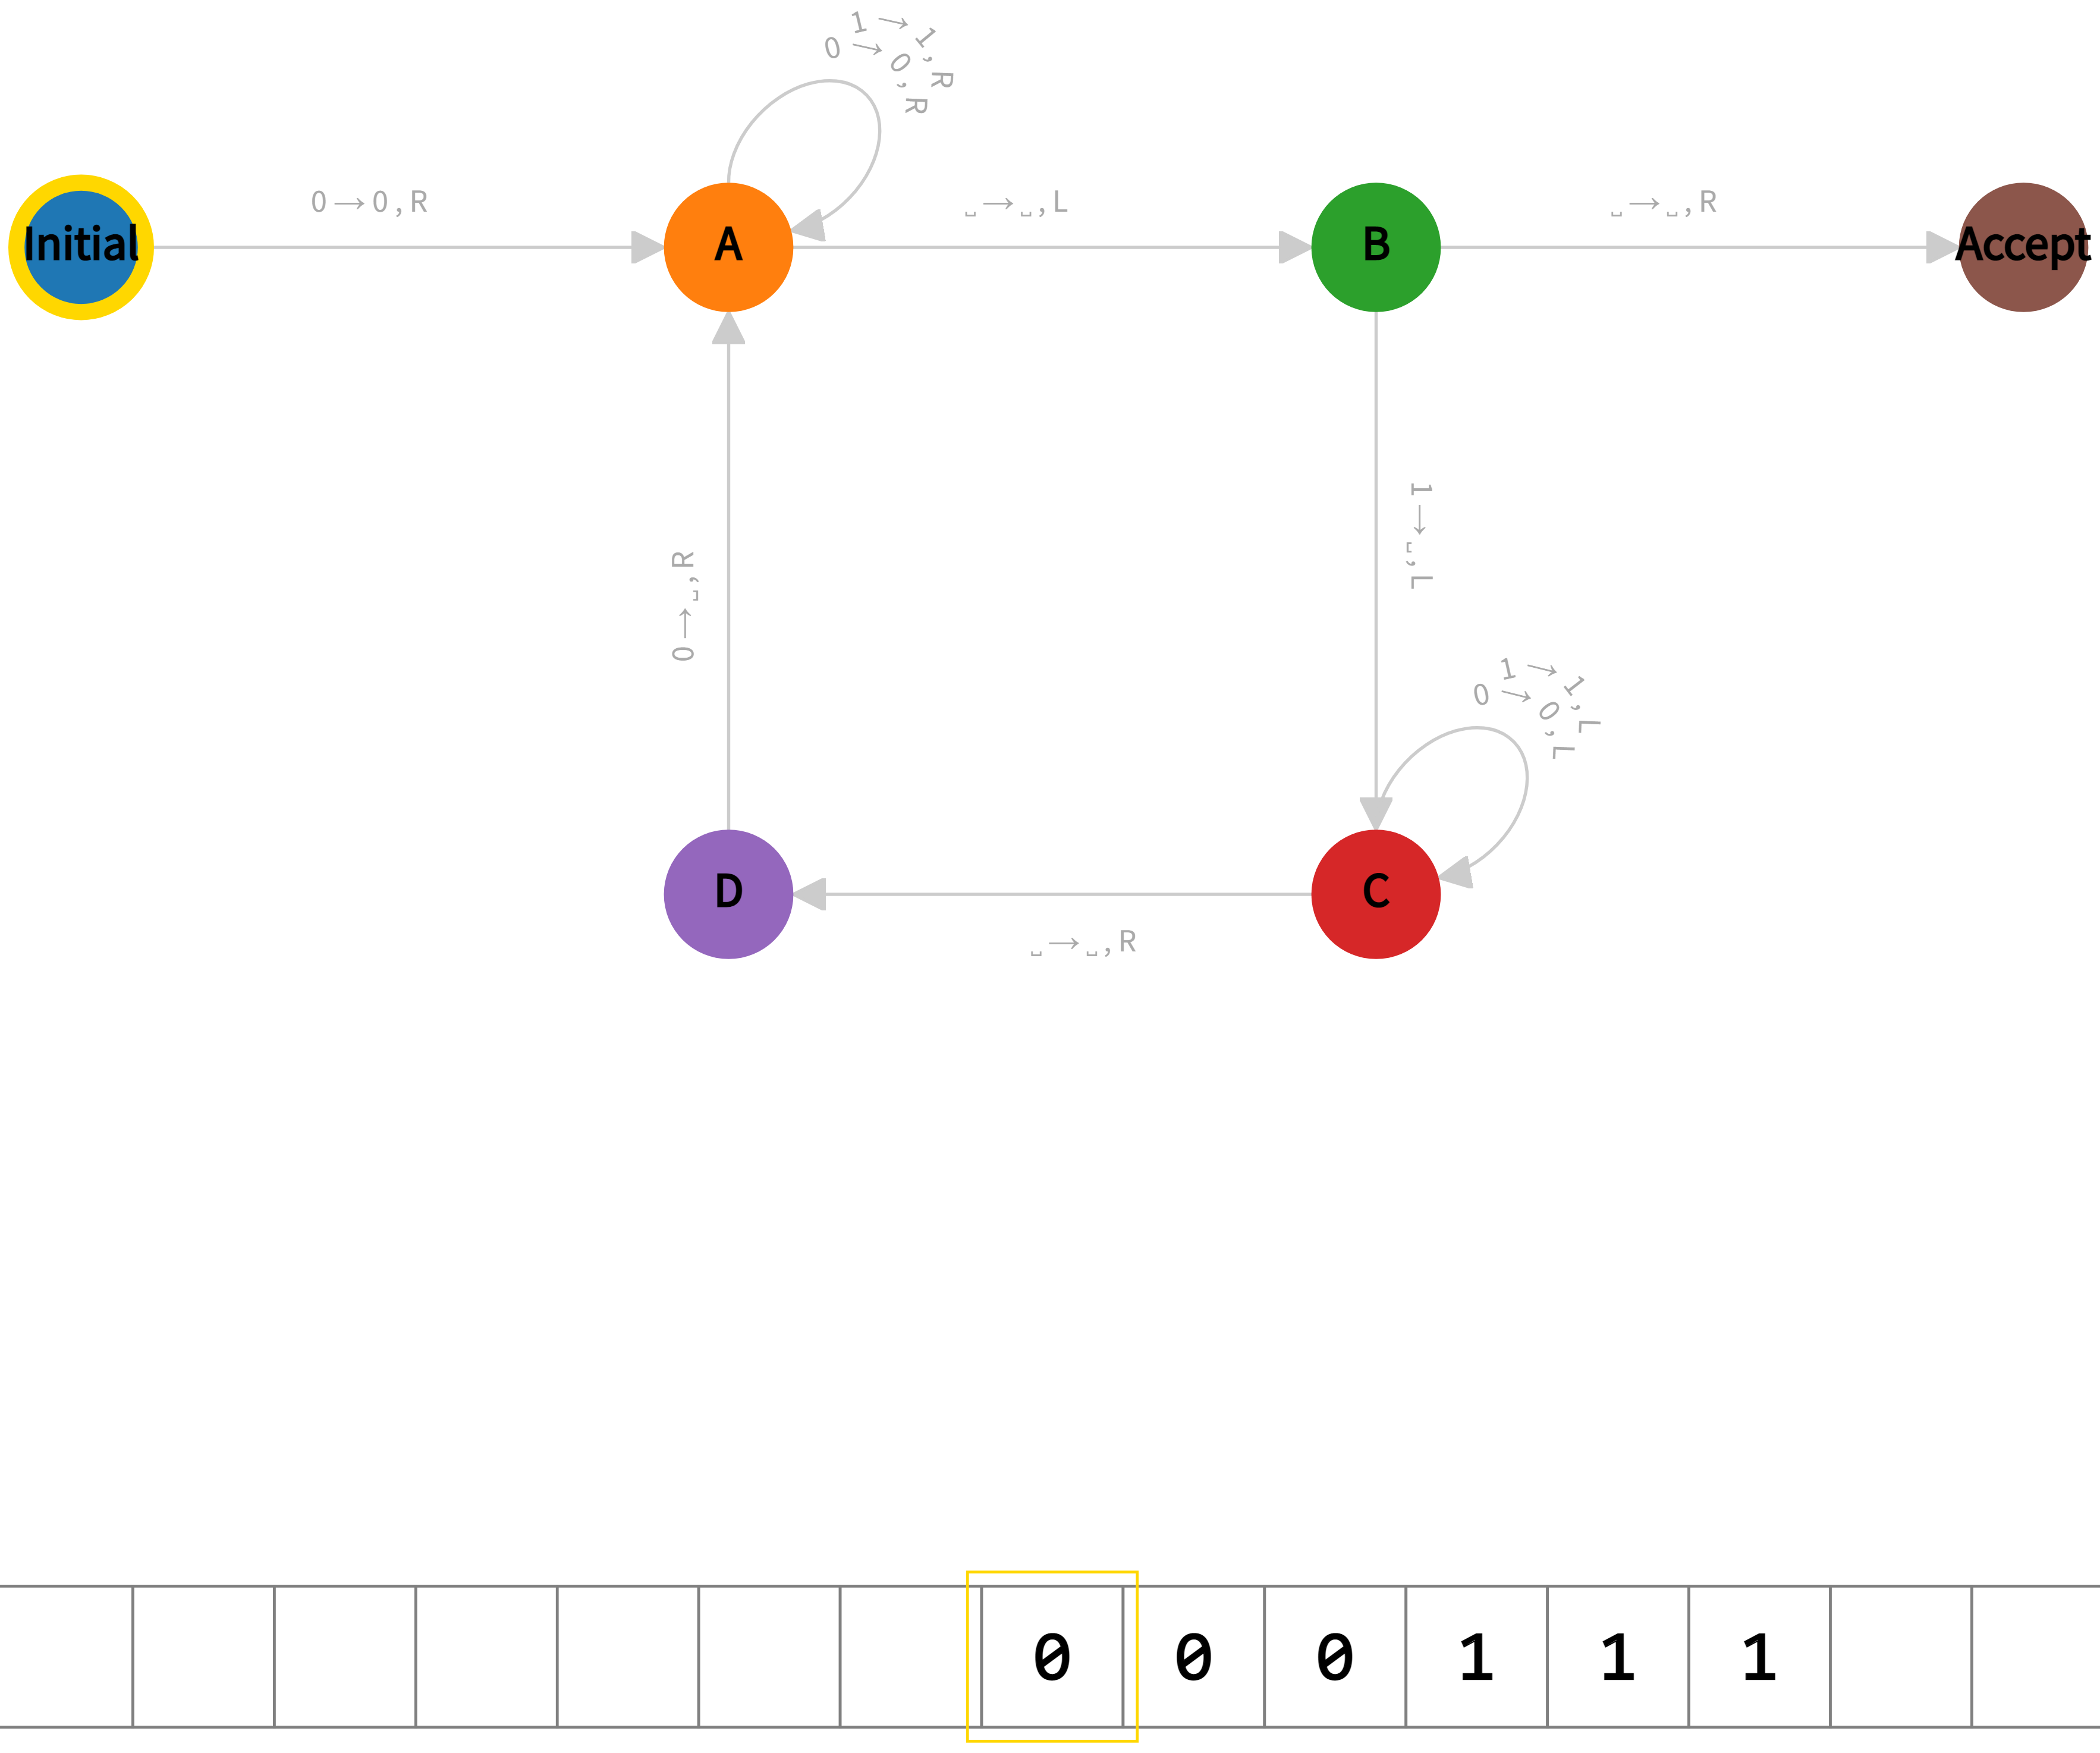
\includegraphics[width=\linewidth]{answers/img/q1-000111-initial.png}
    \caption*{Figure (a): Initial State for $\mathbf{000111}$}
    \label{fig:000111-initial}
  \end{minipage}
  \begin{minipage}{.49\linewidth}
    \centering
    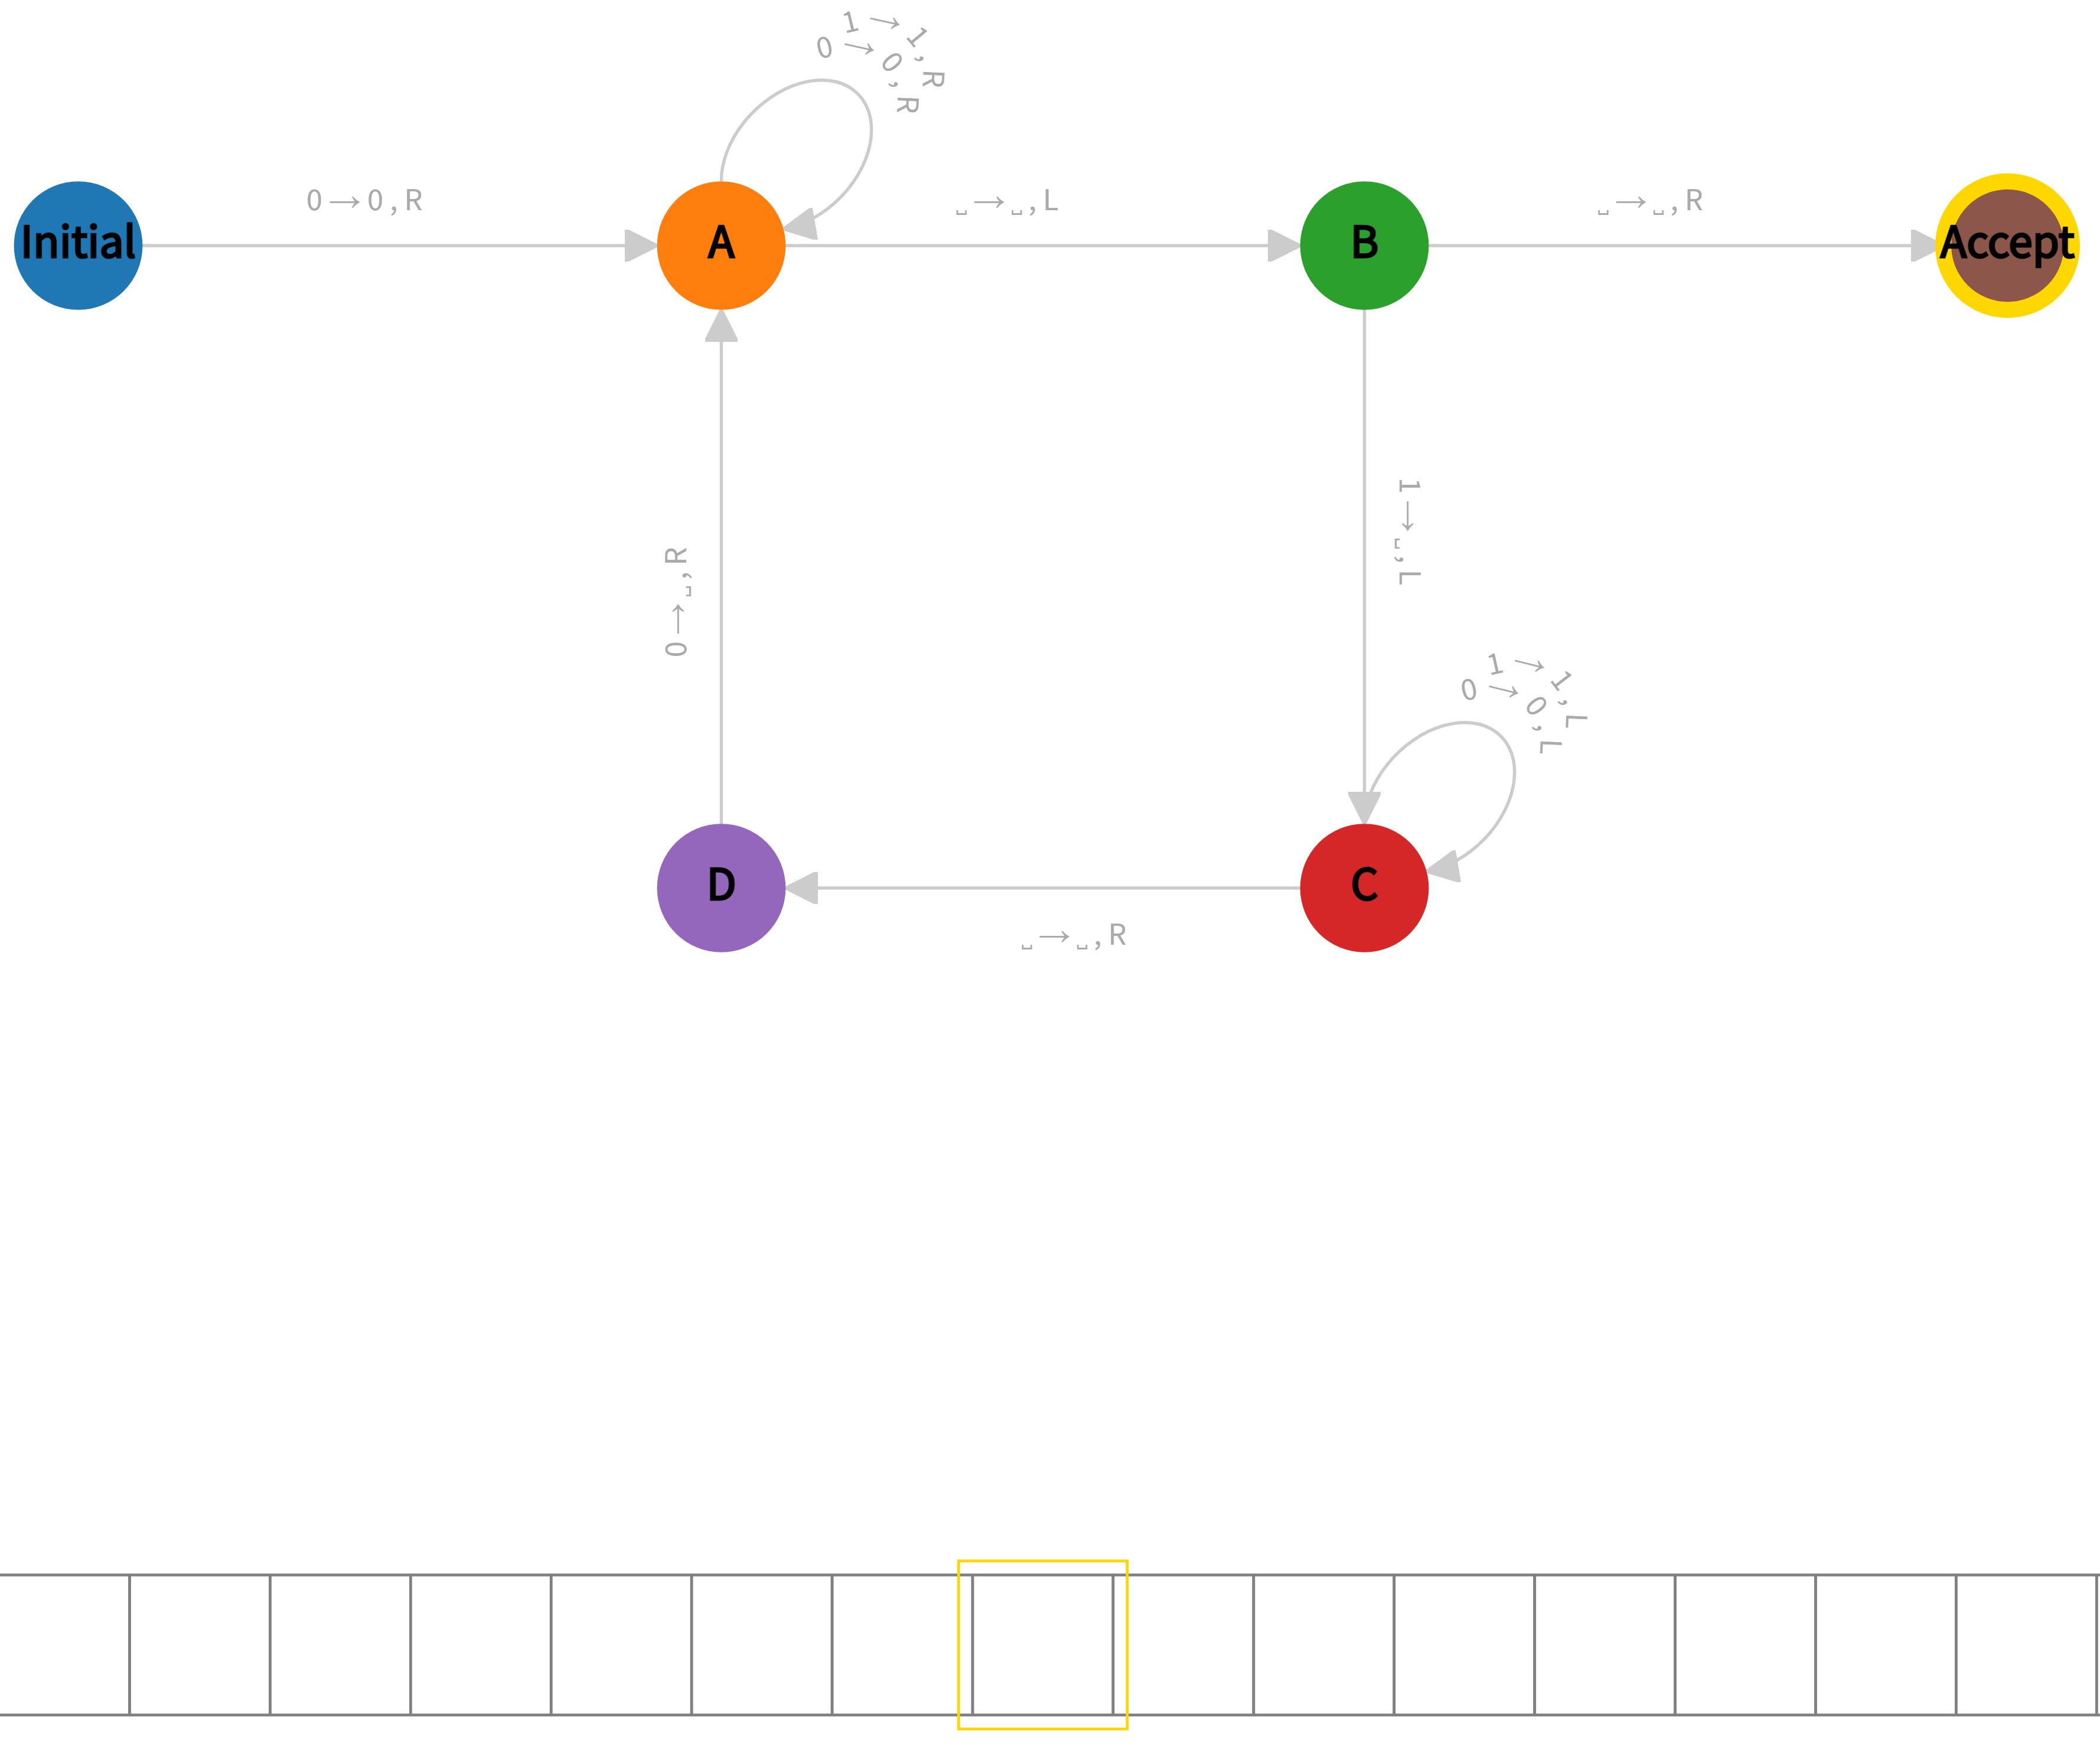
\includegraphics[width=\linewidth]{answers/img/q1-000111-end.png}
    \caption*{Figure (b): End State for $\mathbf{000111}$}
    \label{fig:000111-end}
  \end{minipage}
  \caption{States for $\mathbf{000111}$}
  \label{fig:in-000111}
\end{figure}

\subsubsection*{Input: 0000111 $|$ Reject}
\label{q1-0000111}

\begin{figure}[ht]
  \centering
  \begin{minipage}{.49\linewidth}
    \centering
    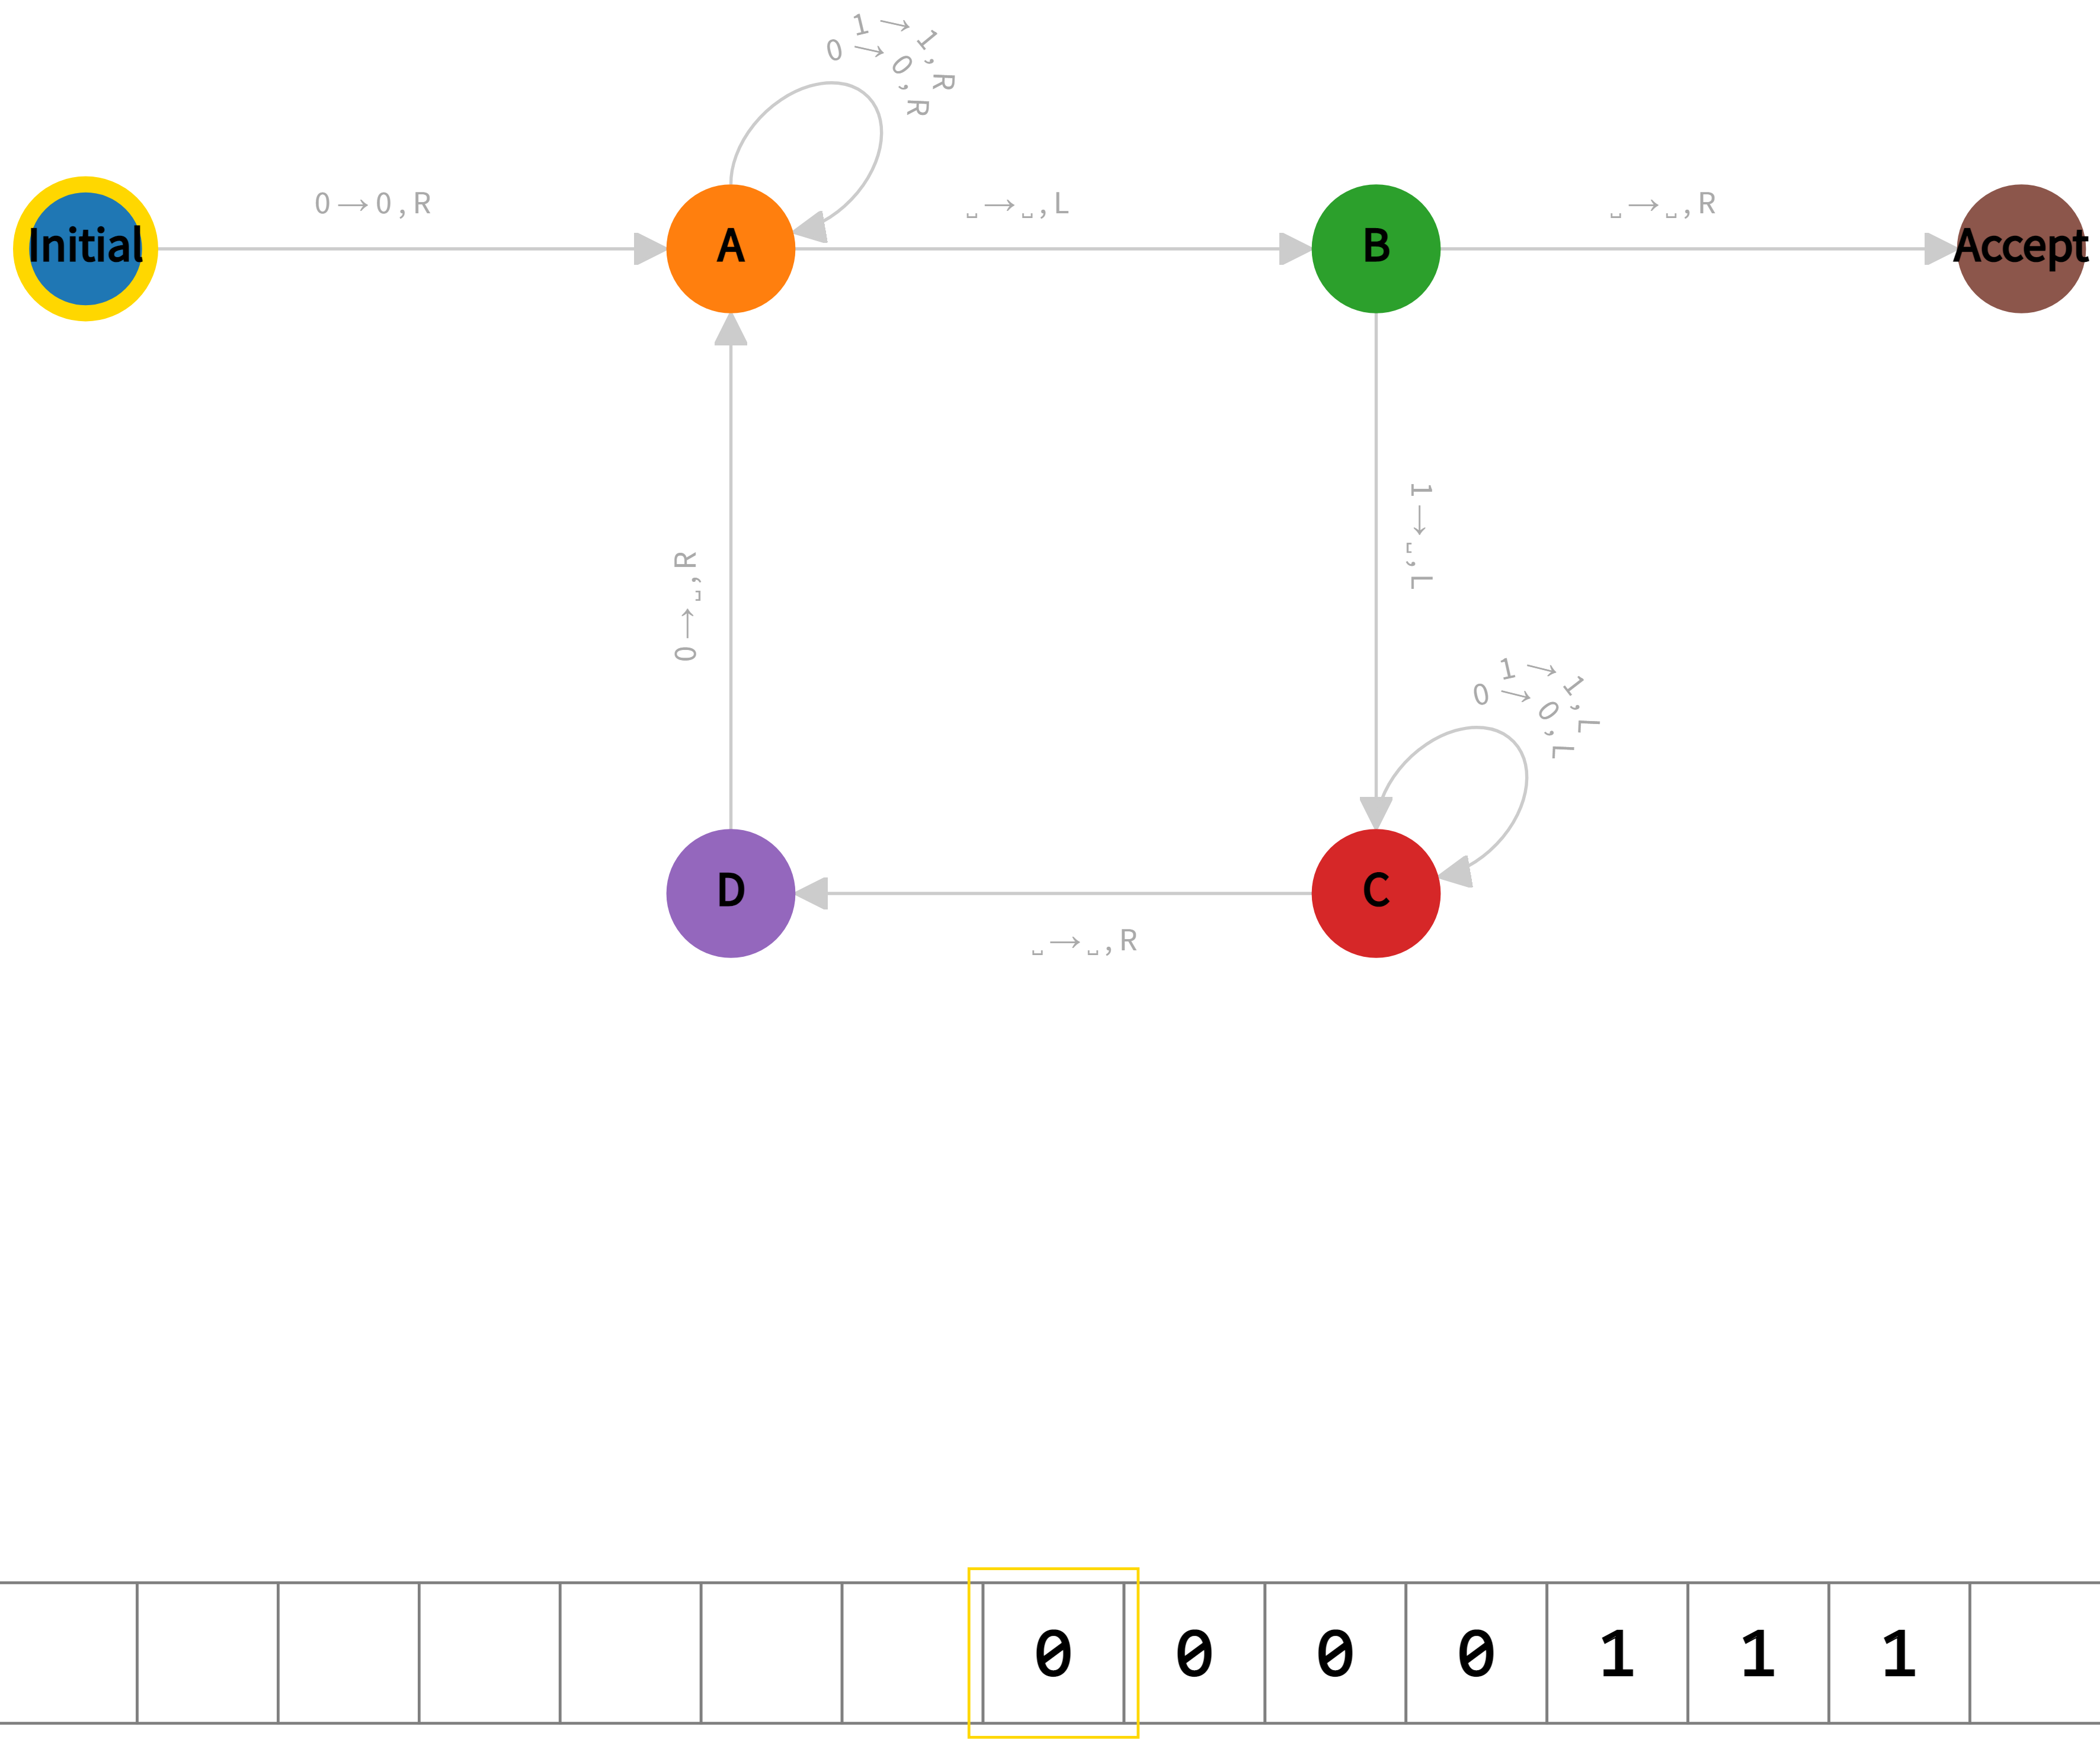
\includegraphics[width=\linewidth]{answers/img/q1-0000111-initial.png}
    \caption*{Figure (a): Initial State for $\mathbf{0000111}$}
    \label{fig:0000111-initial}
  \end{minipage}
  \begin{minipage}{.49\linewidth}
    \centering
    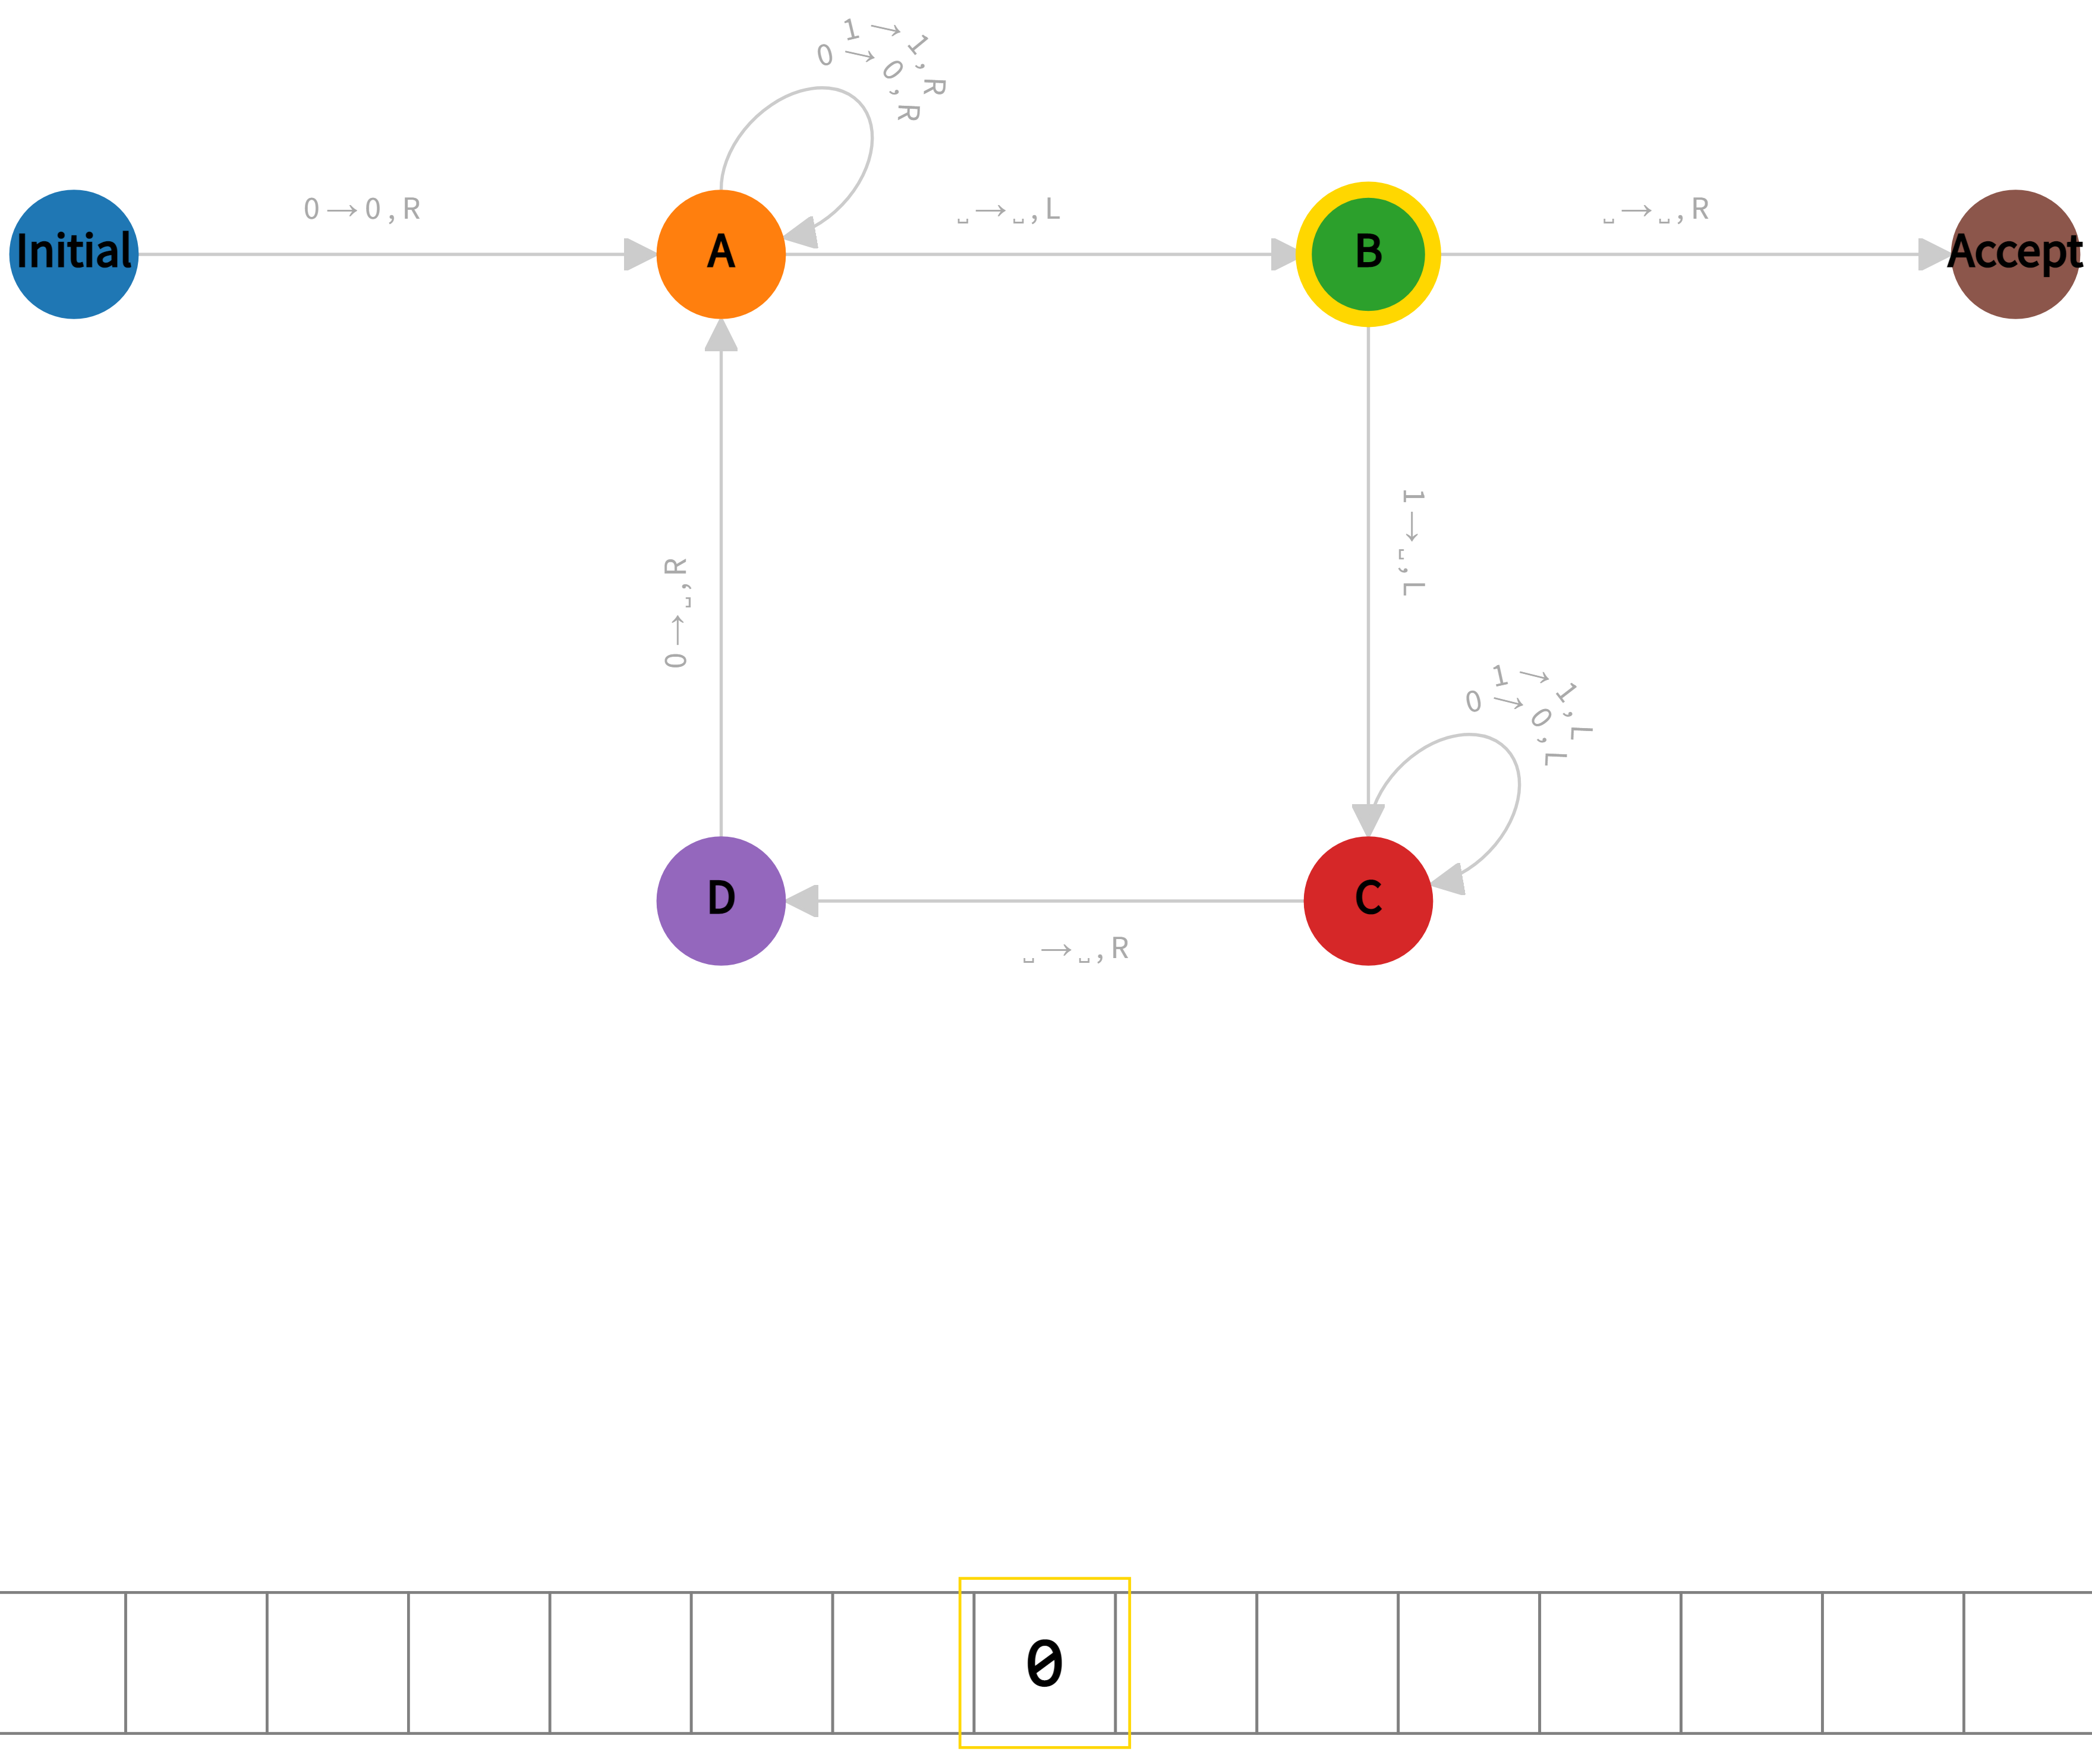
\includegraphics[width=\linewidth]{answers/img/q1-0000111-end.png}
    \caption*{Figure (b): End State for $\mathbf{0000111}$}
    \label{fig:0000111-end}
  \end{minipage}
  \caption{States for $\mathbf{0000111}$}
  \label{fig:in-0000111}
\end{figure}

\vspace*{\fill}
\newpage
\vspace*{\fill}

\subsubsection*{Input: 000011111 $|$ Reject}
\label{q1-000011111}

\begin{figure}[ht]
  \centering
  \begin{minipage}{.49\linewidth}
    \centering
    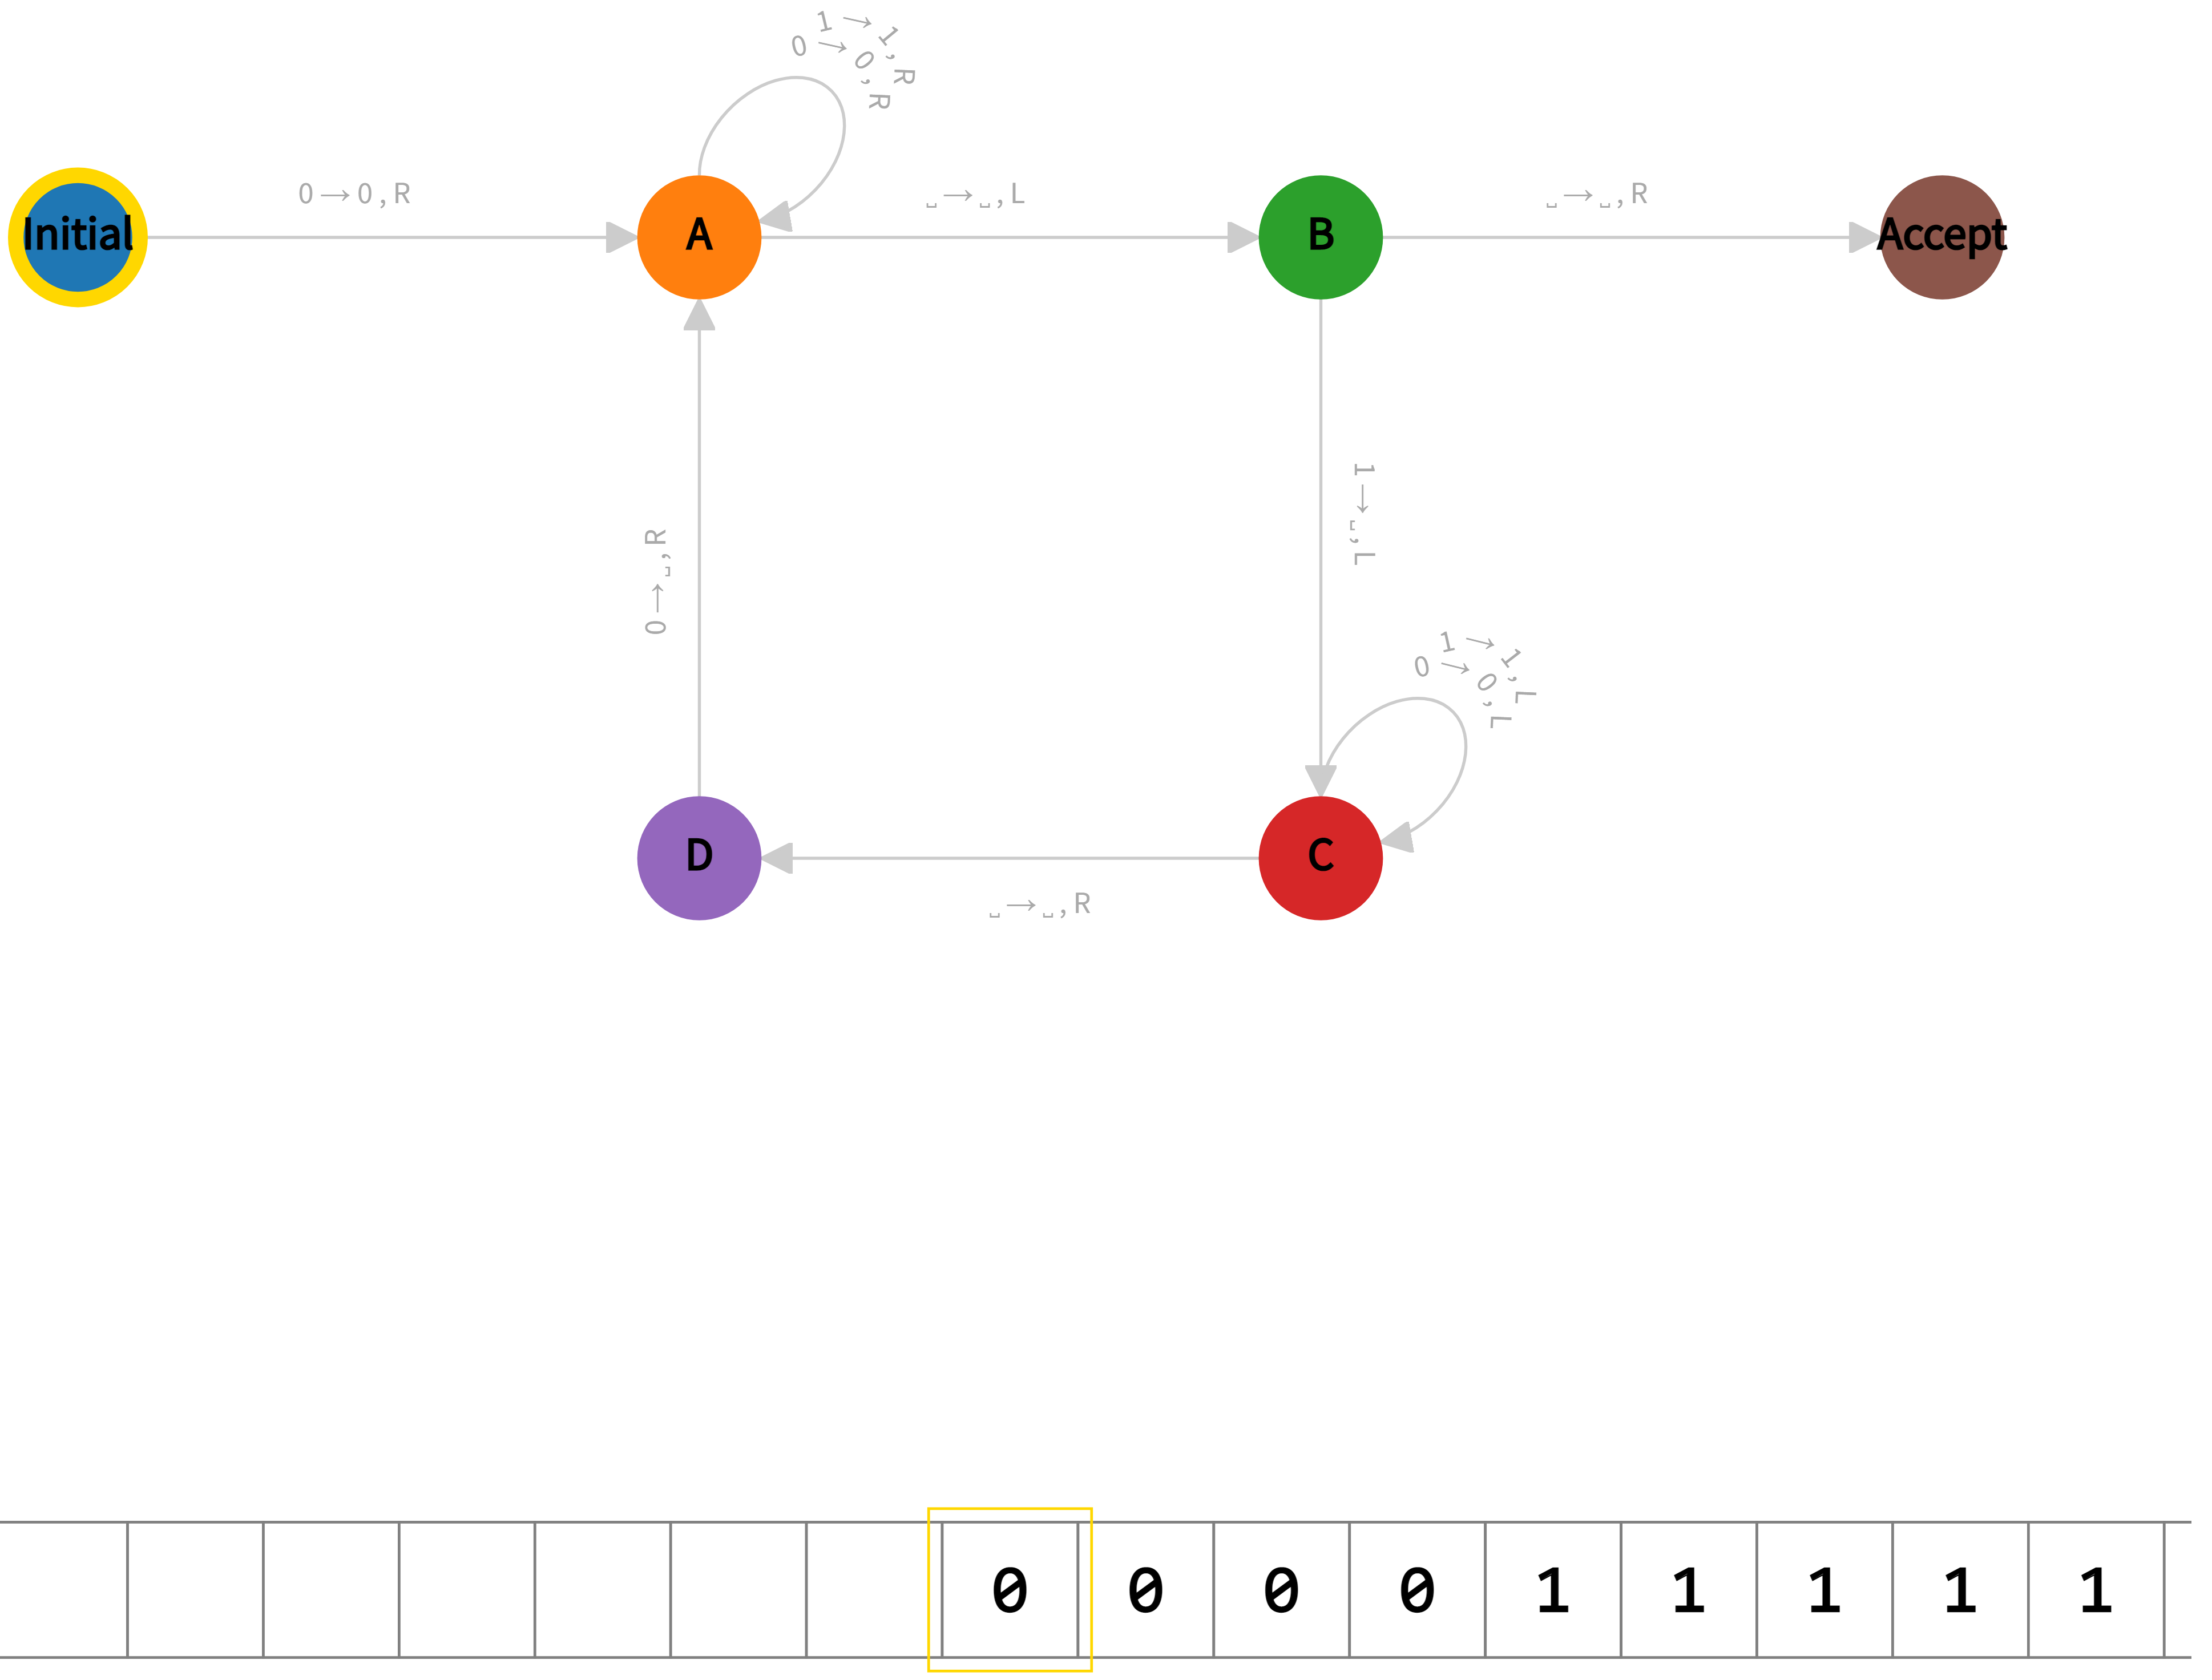
\includegraphics[width=\linewidth]{answers/img/q1-000011111-initial.png}
    \caption*{Figure (a): Initial State for $\mathbf{000011111}$}
    \label{fig:000011111-initial}
  \end{minipage}
  \begin{minipage}{.49\linewidth}
    \centering
    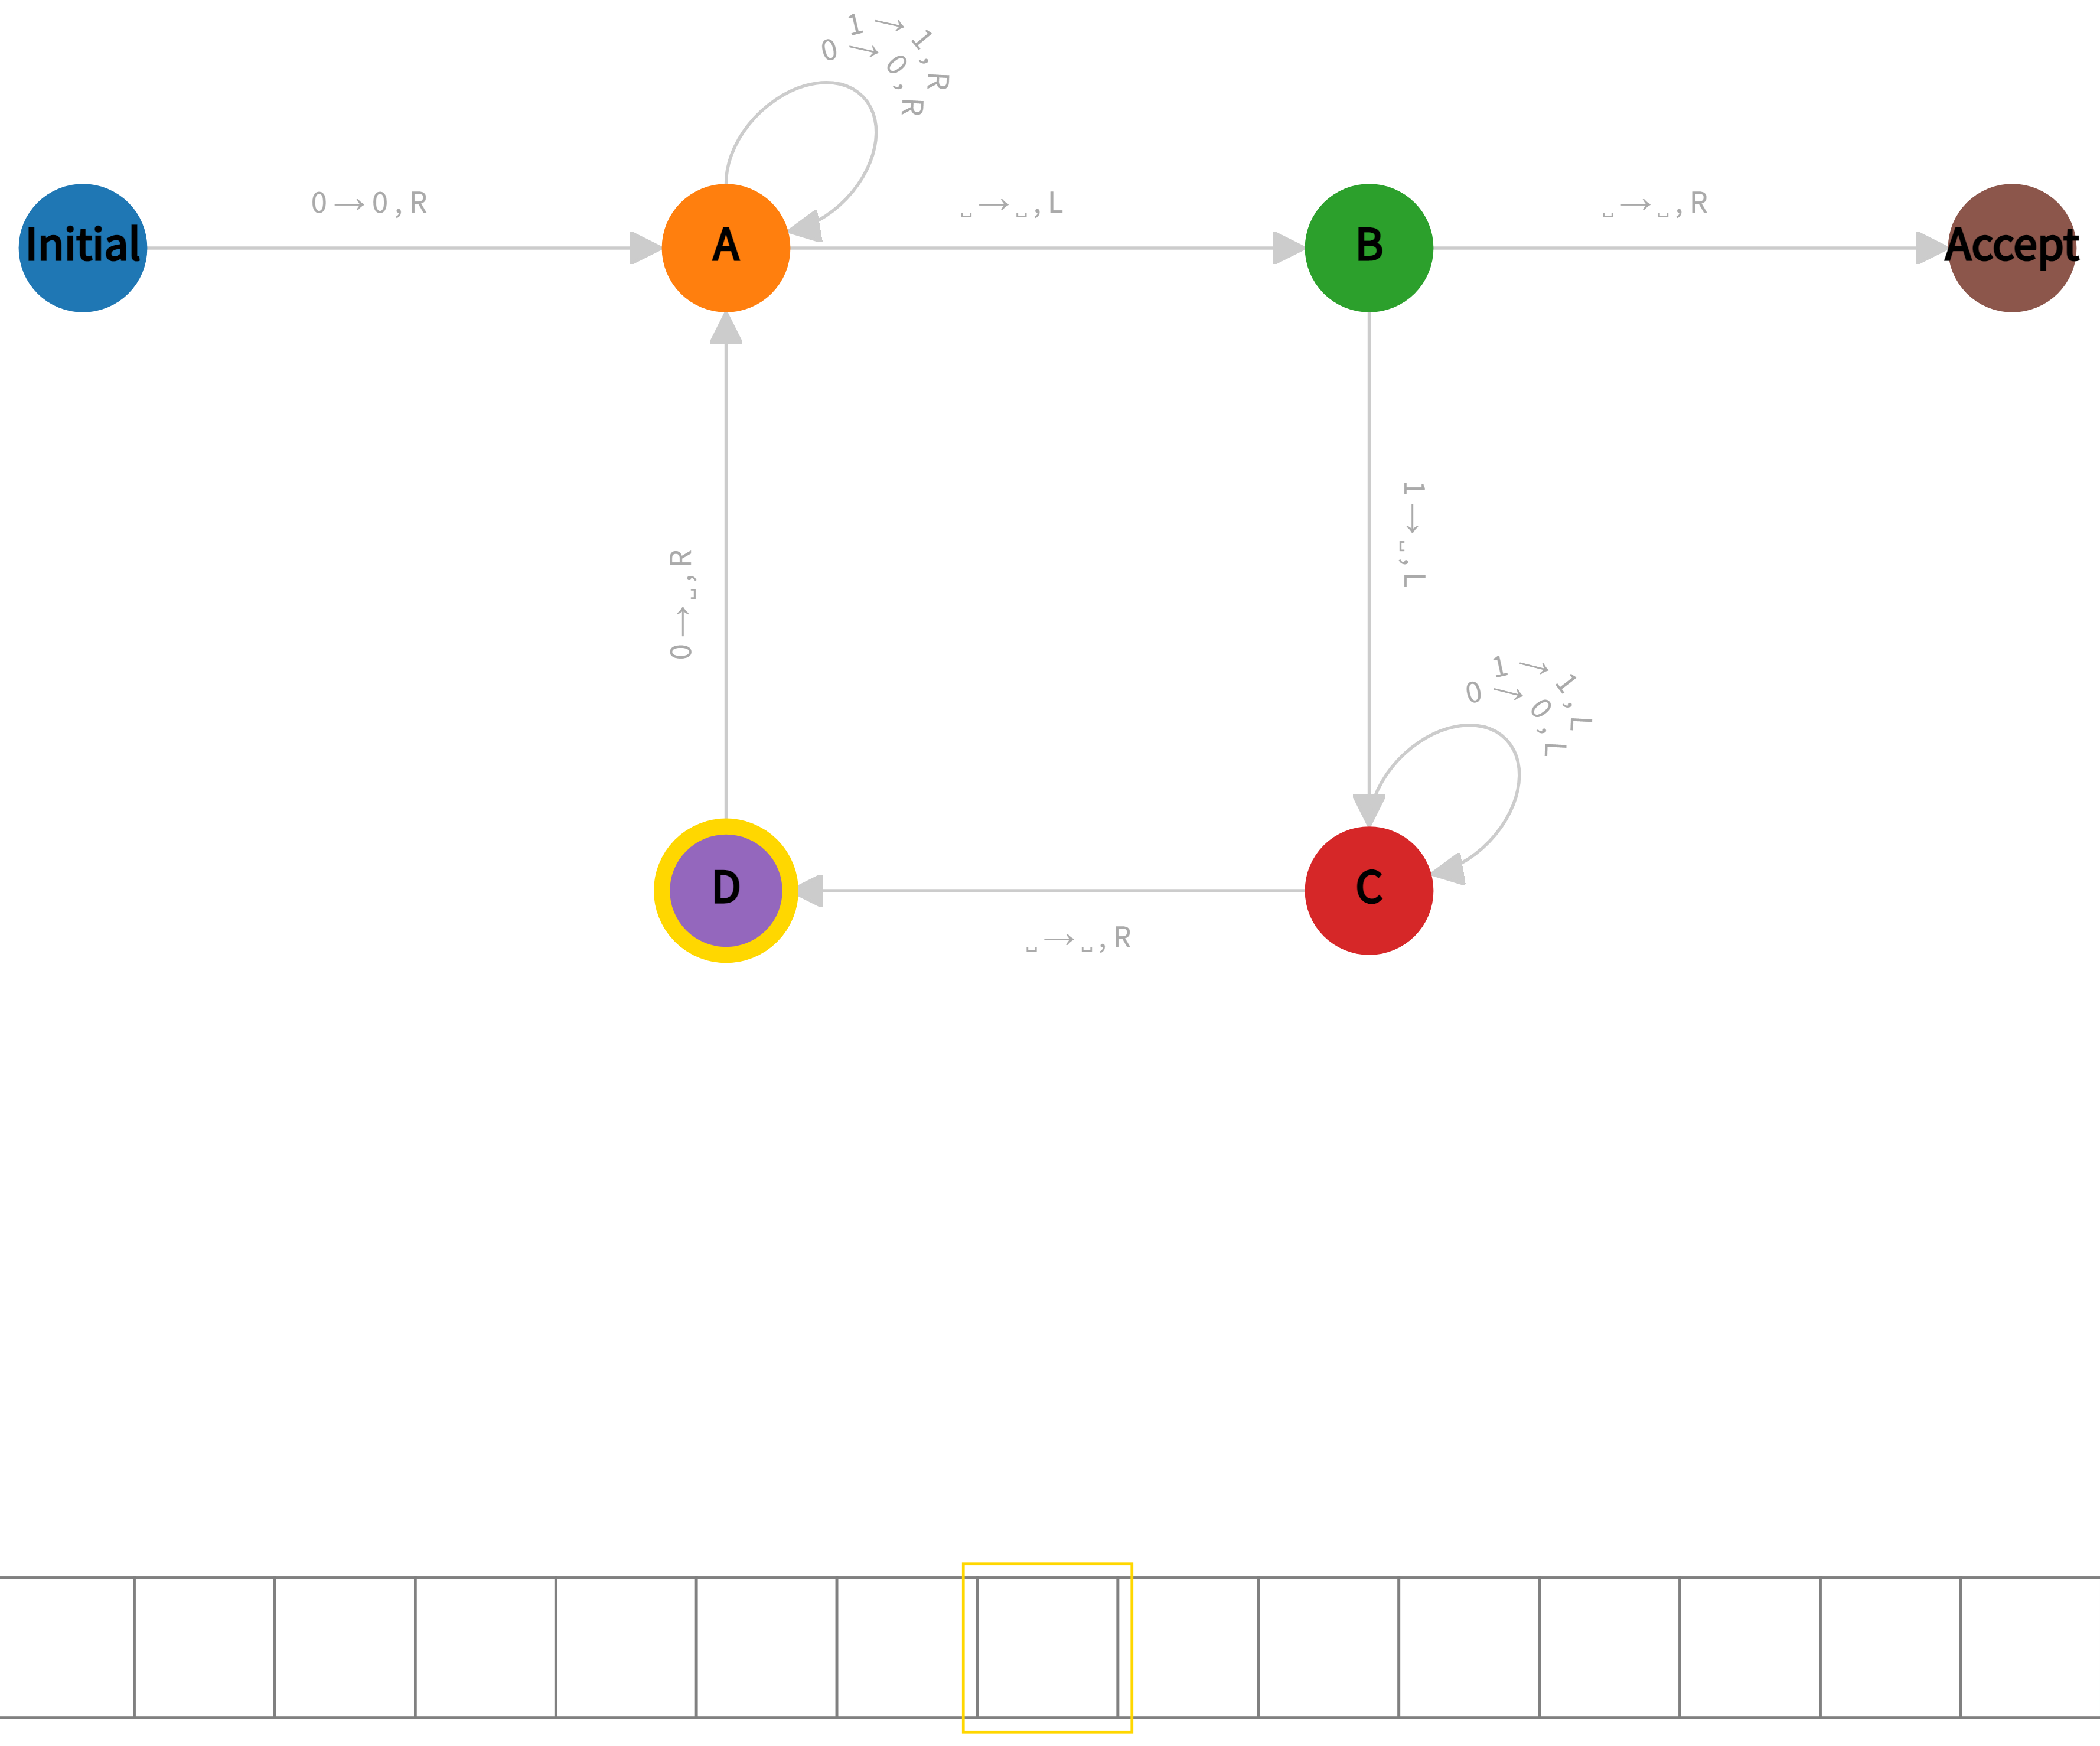
\includegraphics[width=\linewidth]{answers/img/q1-000011111-end.png}
    \caption*{Figure (b): End State for $\mathbf{000011111}$}
    \label{fig:000011111-end}
  \end{minipage}
  \caption{States for $\mathbf{000011111}$}
  \label{fig:in-000011111}
\end{figure}

\subsubsection*{Input: 0001110 $|$ Reject}
\label{q1-0001110}

\begin{figure}[ht]
  \centering
  \begin{minipage}{.49\linewidth}
    \centering
    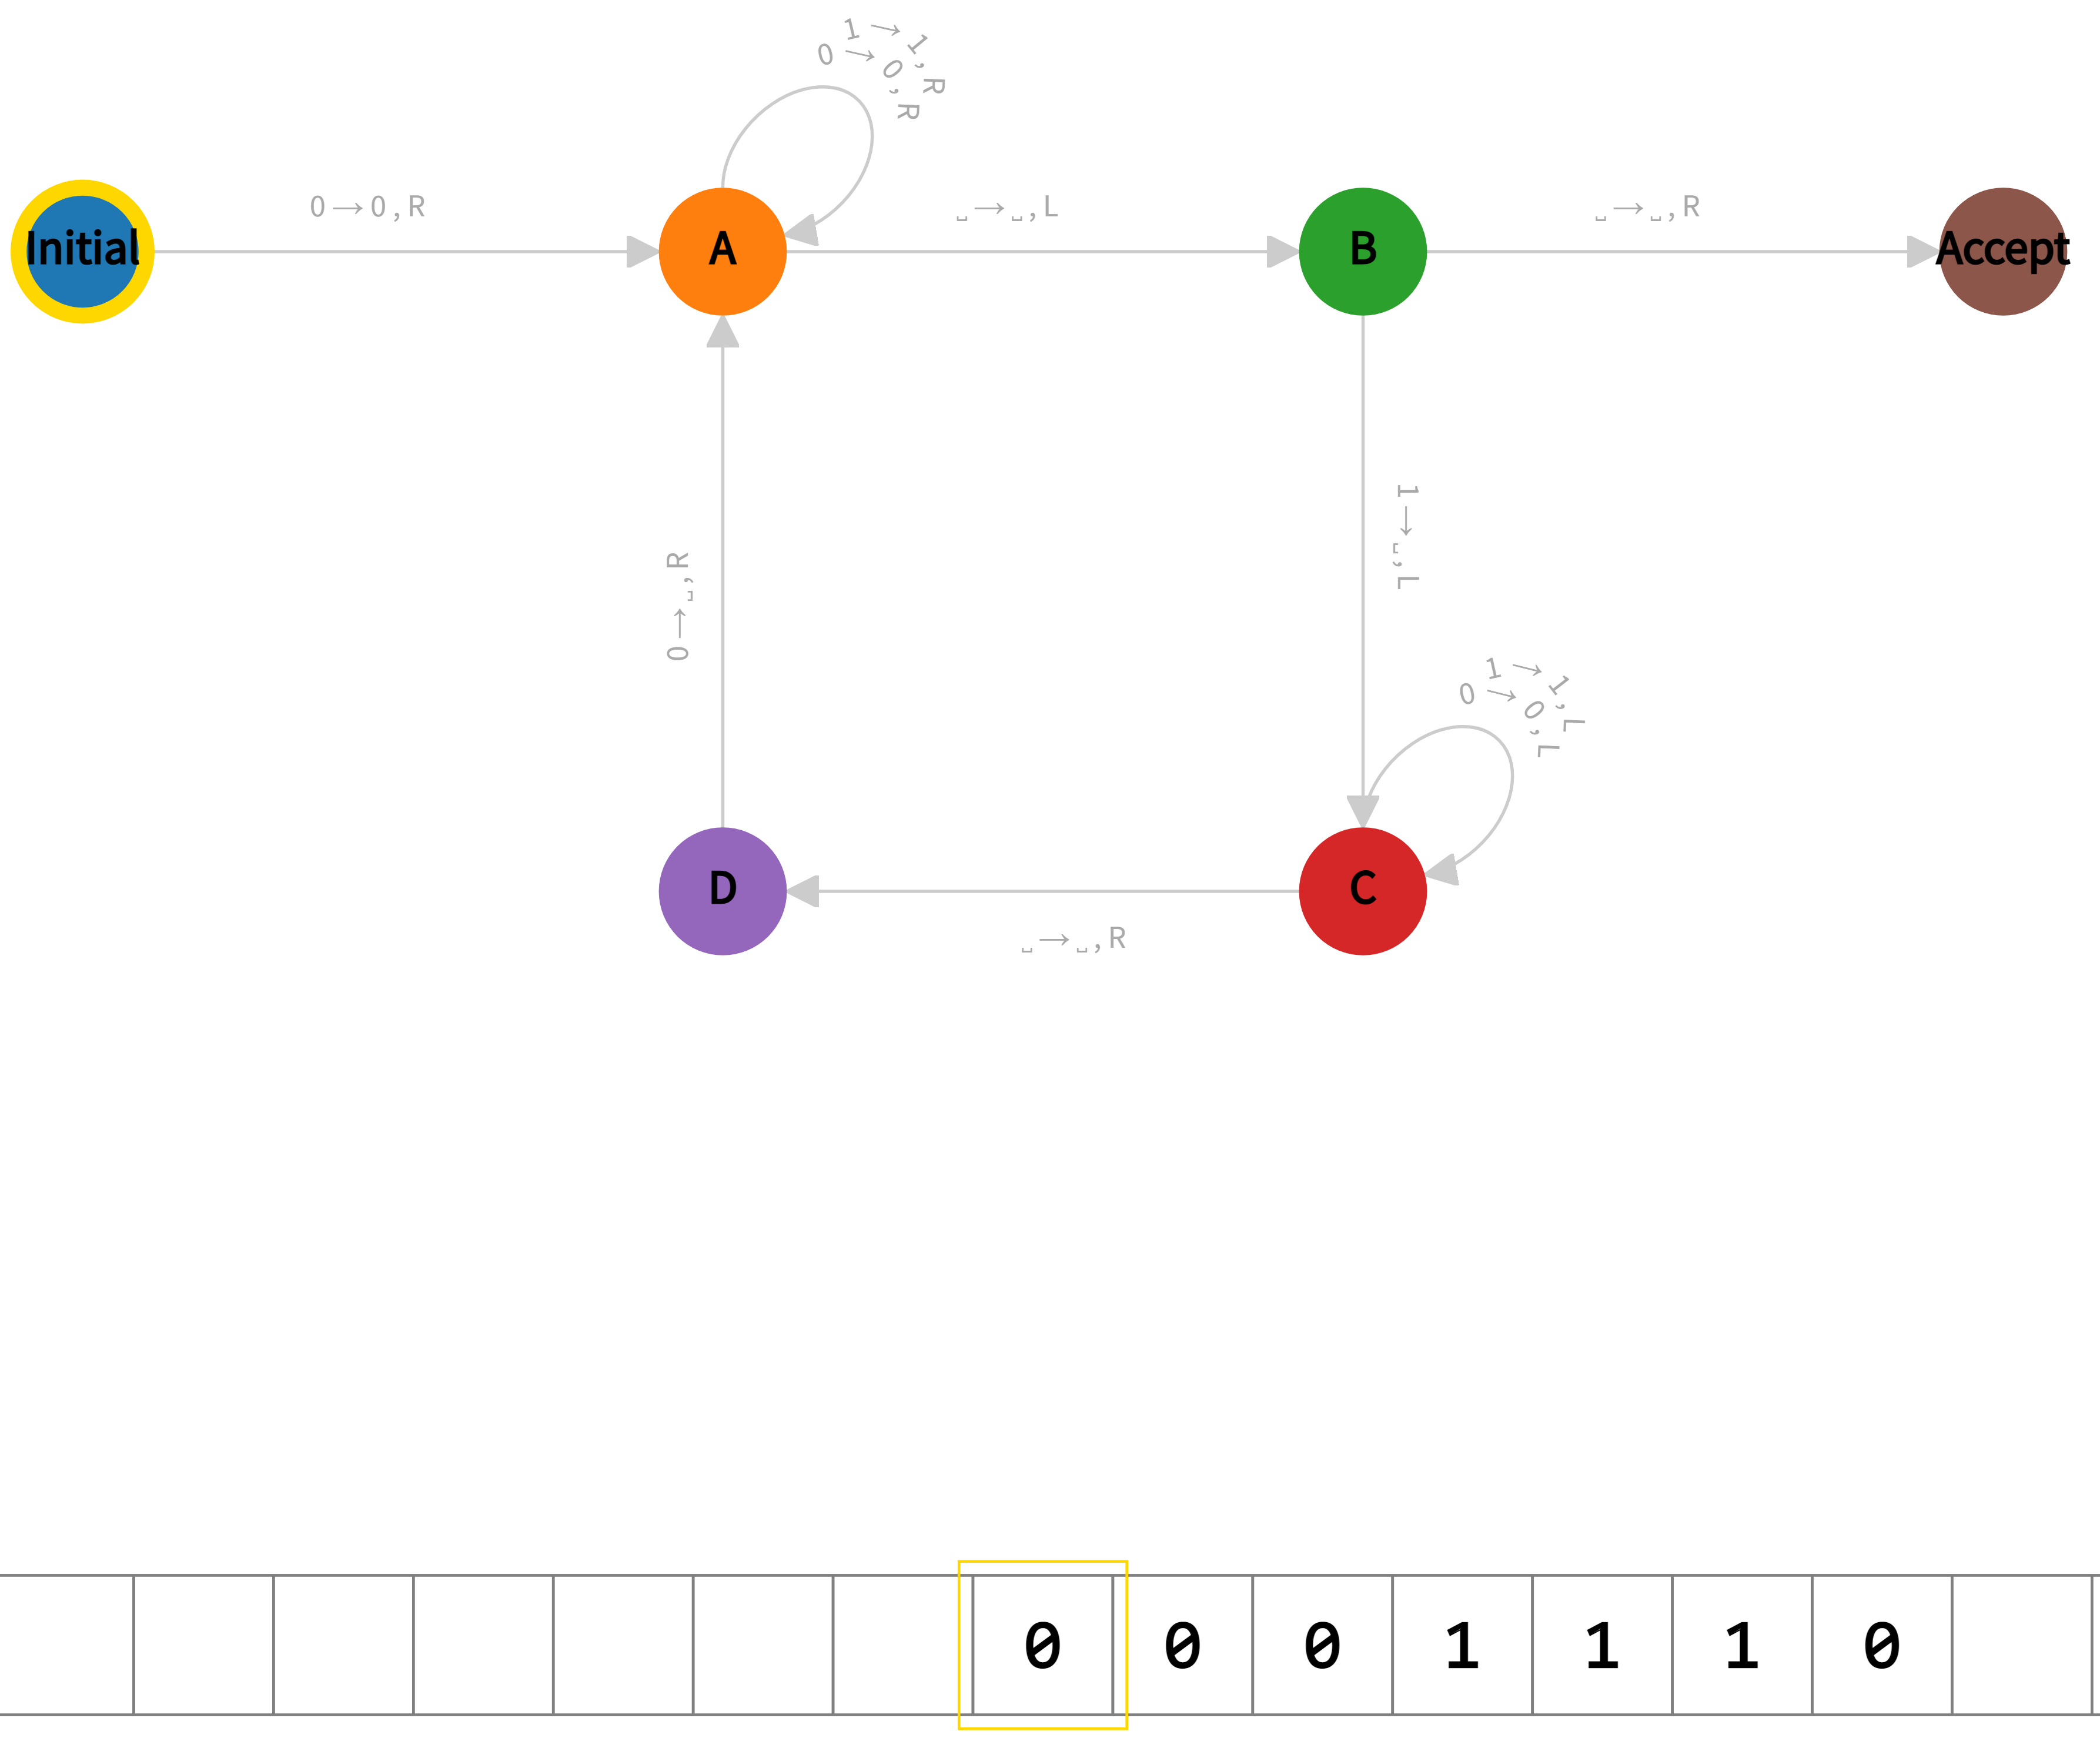
\includegraphics[width=\linewidth]{answers/img/q1-0001110-initial.png}
    \caption*{Figure (a): Initial State for $\mathbf{0001110}$}
    \label{fig:0001110-initial}
  \end{minipage}
  \begin{minipage}{.49\linewidth}
    \centering
    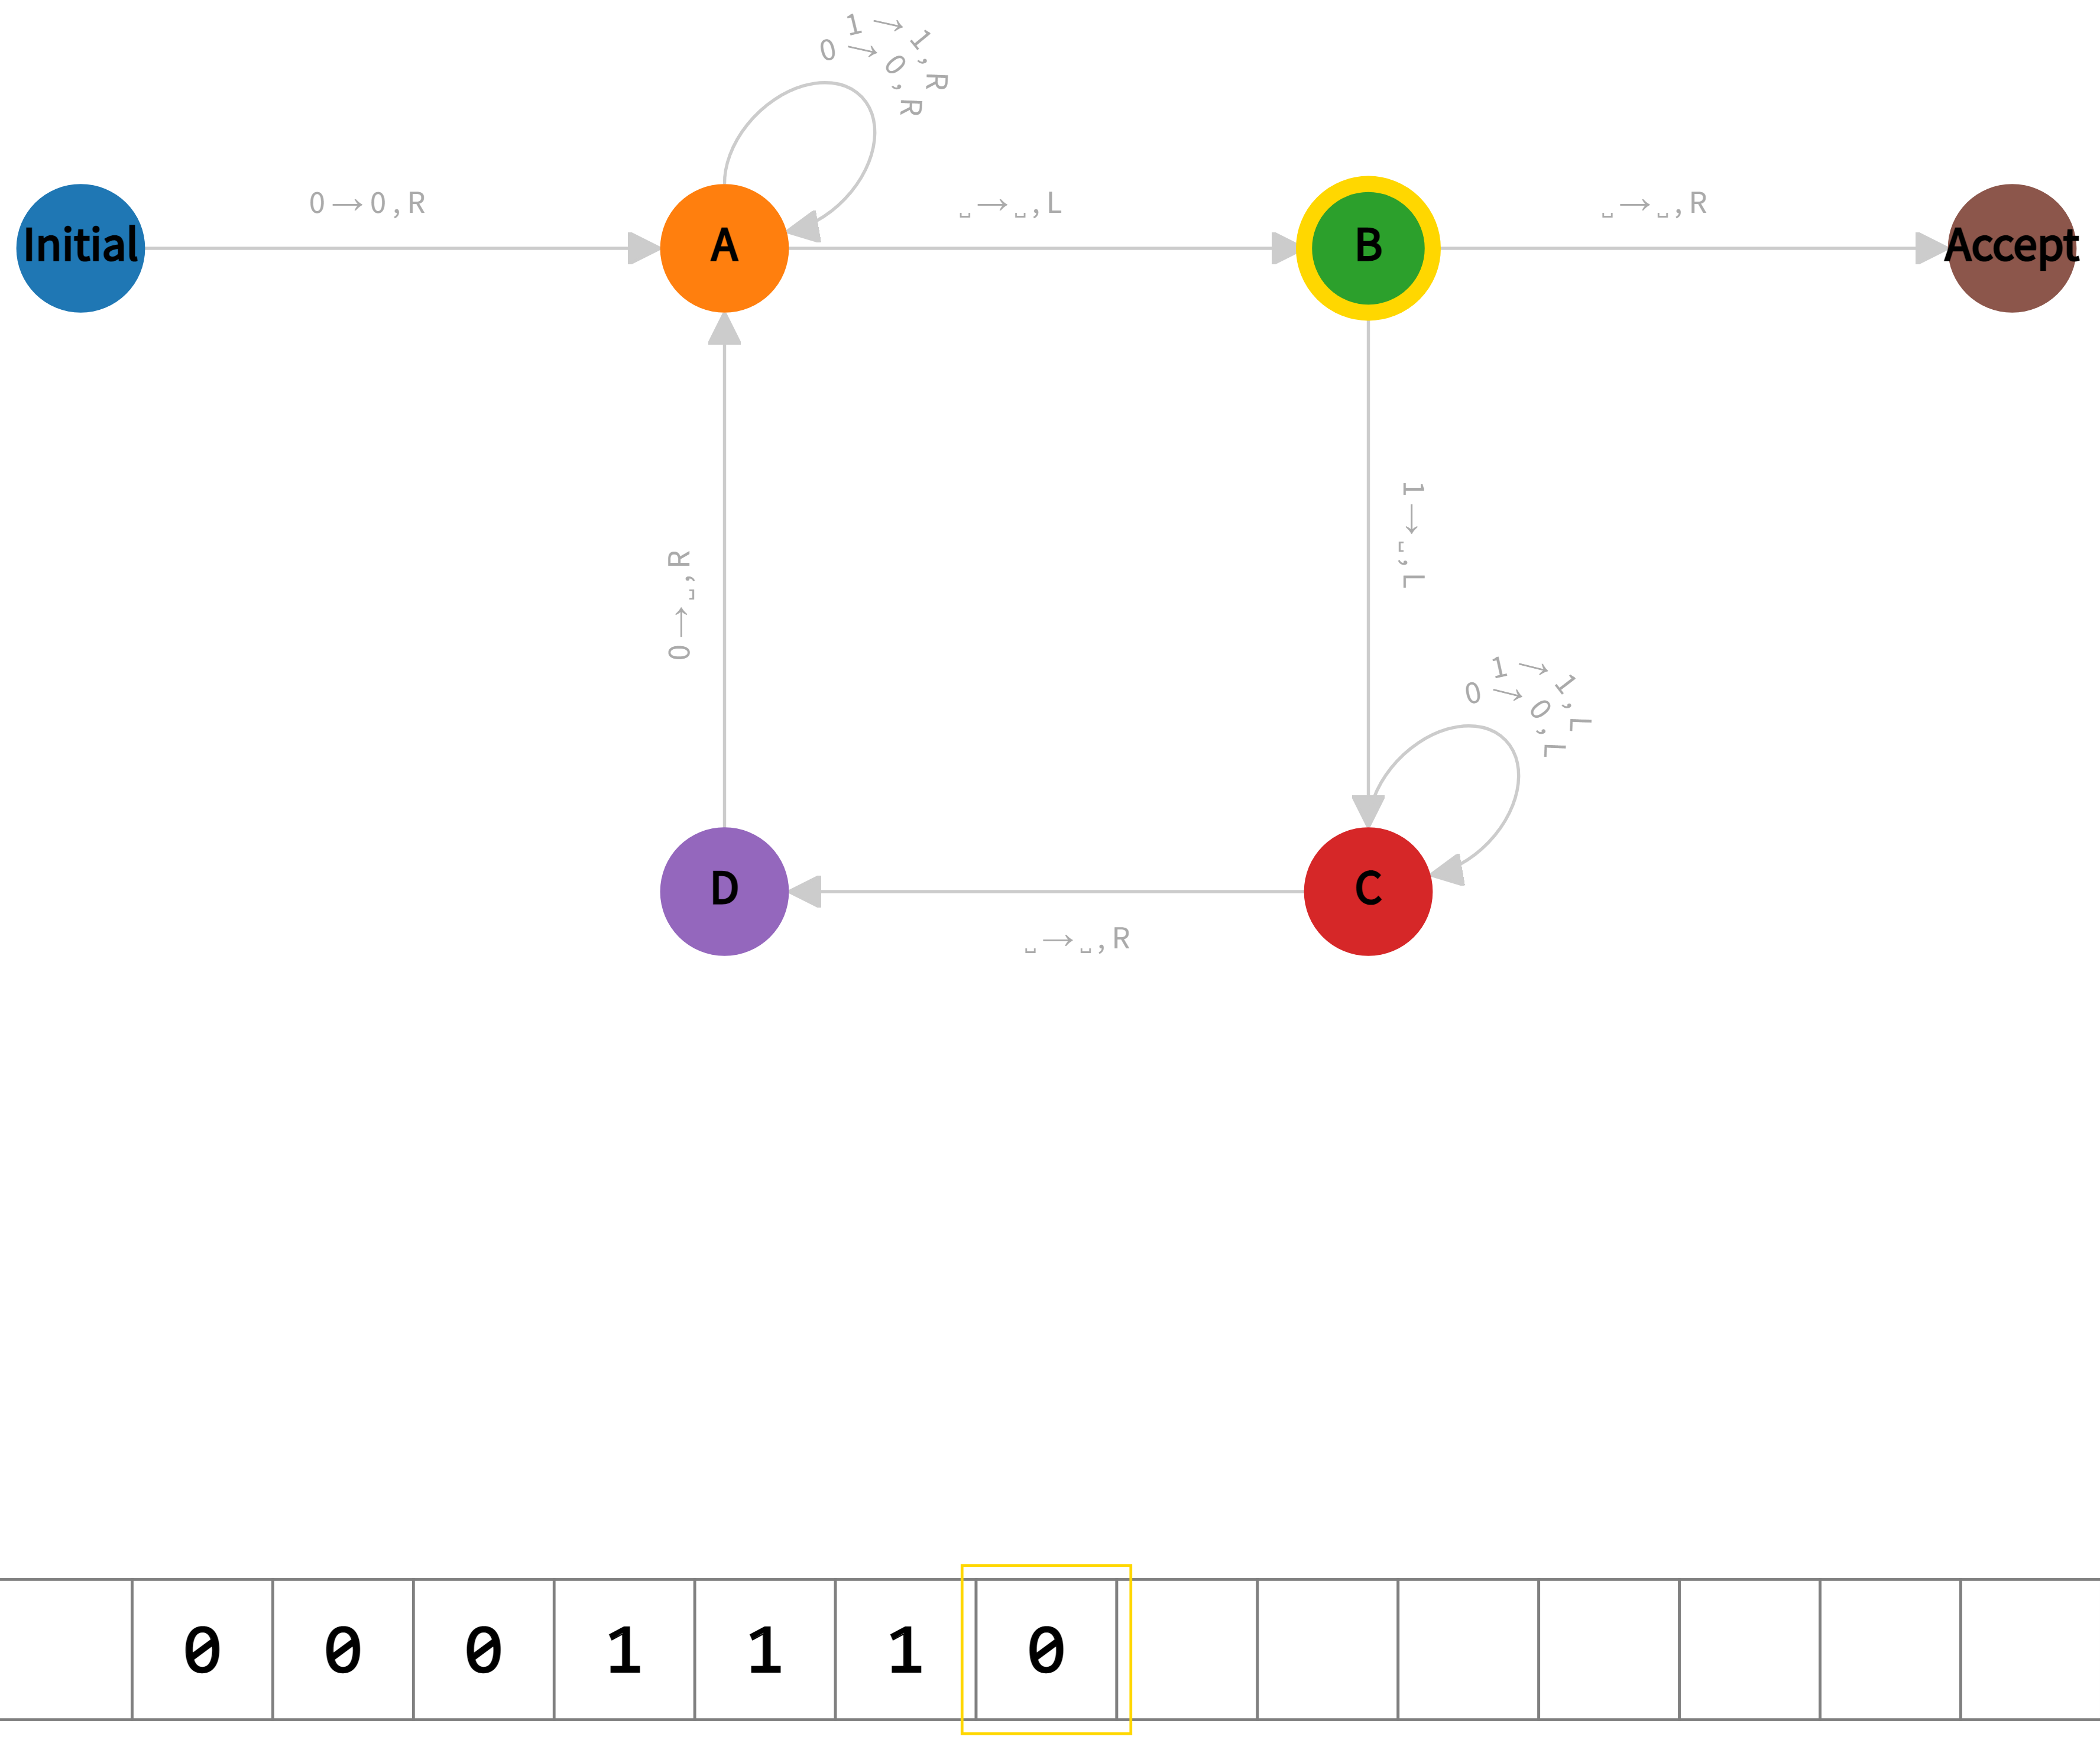
\includegraphics[width=\linewidth]{answers/img/q1-0001110-end.png}
    \caption*{Figure (b): End State for $\mathbf{0001110}$}
    \label{fig:0001110-end}
  \end{minipage}
  \caption{States for $\mathbf{0001110}$}
  \label{fig:in-0001110}
\end{figure}

\vspace*{\fill}
\newpage
\vspace*{\fill}

\subsubsection*{Input: 001101 $|$ Reject}
\label{q1-001101}

\begin{figure}[ht]
  \centering
  \begin{minipage}{.49\linewidth}
    \centering
    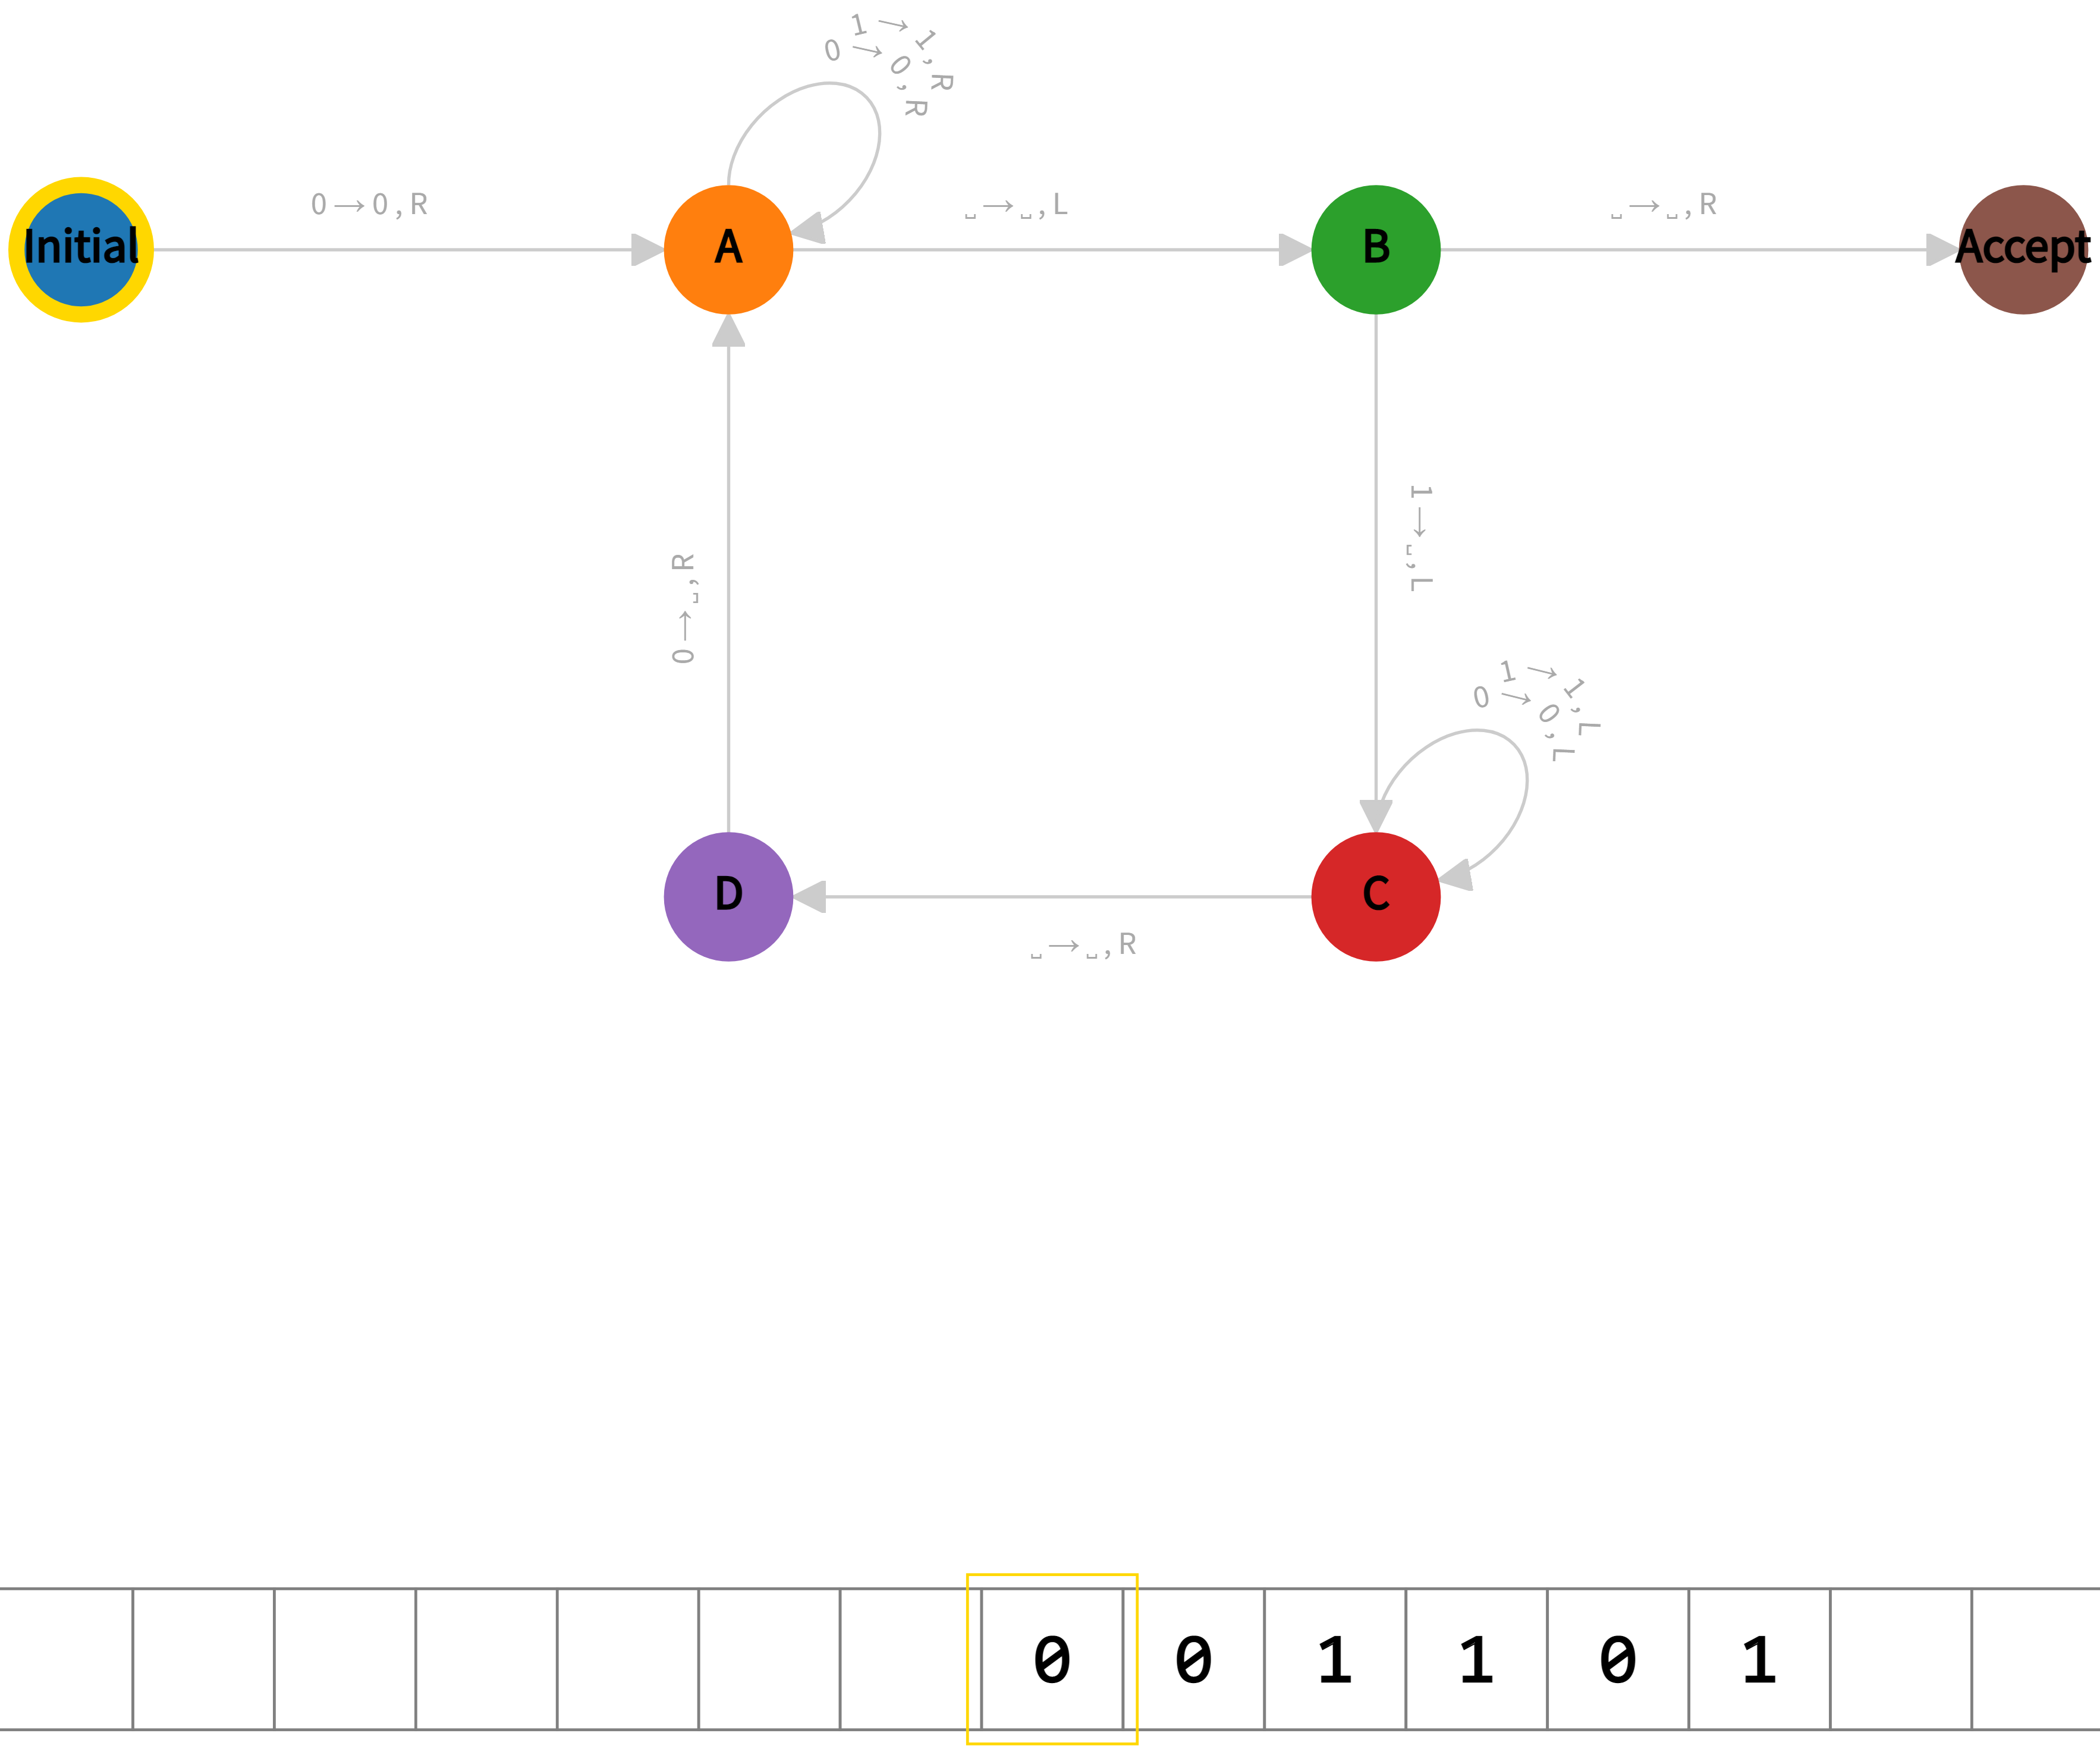
\includegraphics[width=\linewidth]{answers/img/q1-001101-initial.png}
    \caption*{Figure (a): Initial State for $\mathbf{001101}$}
    \label{fig:001101-initial}
  \end{minipage}
  \begin{minipage}{.49\linewidth}
    \centering
    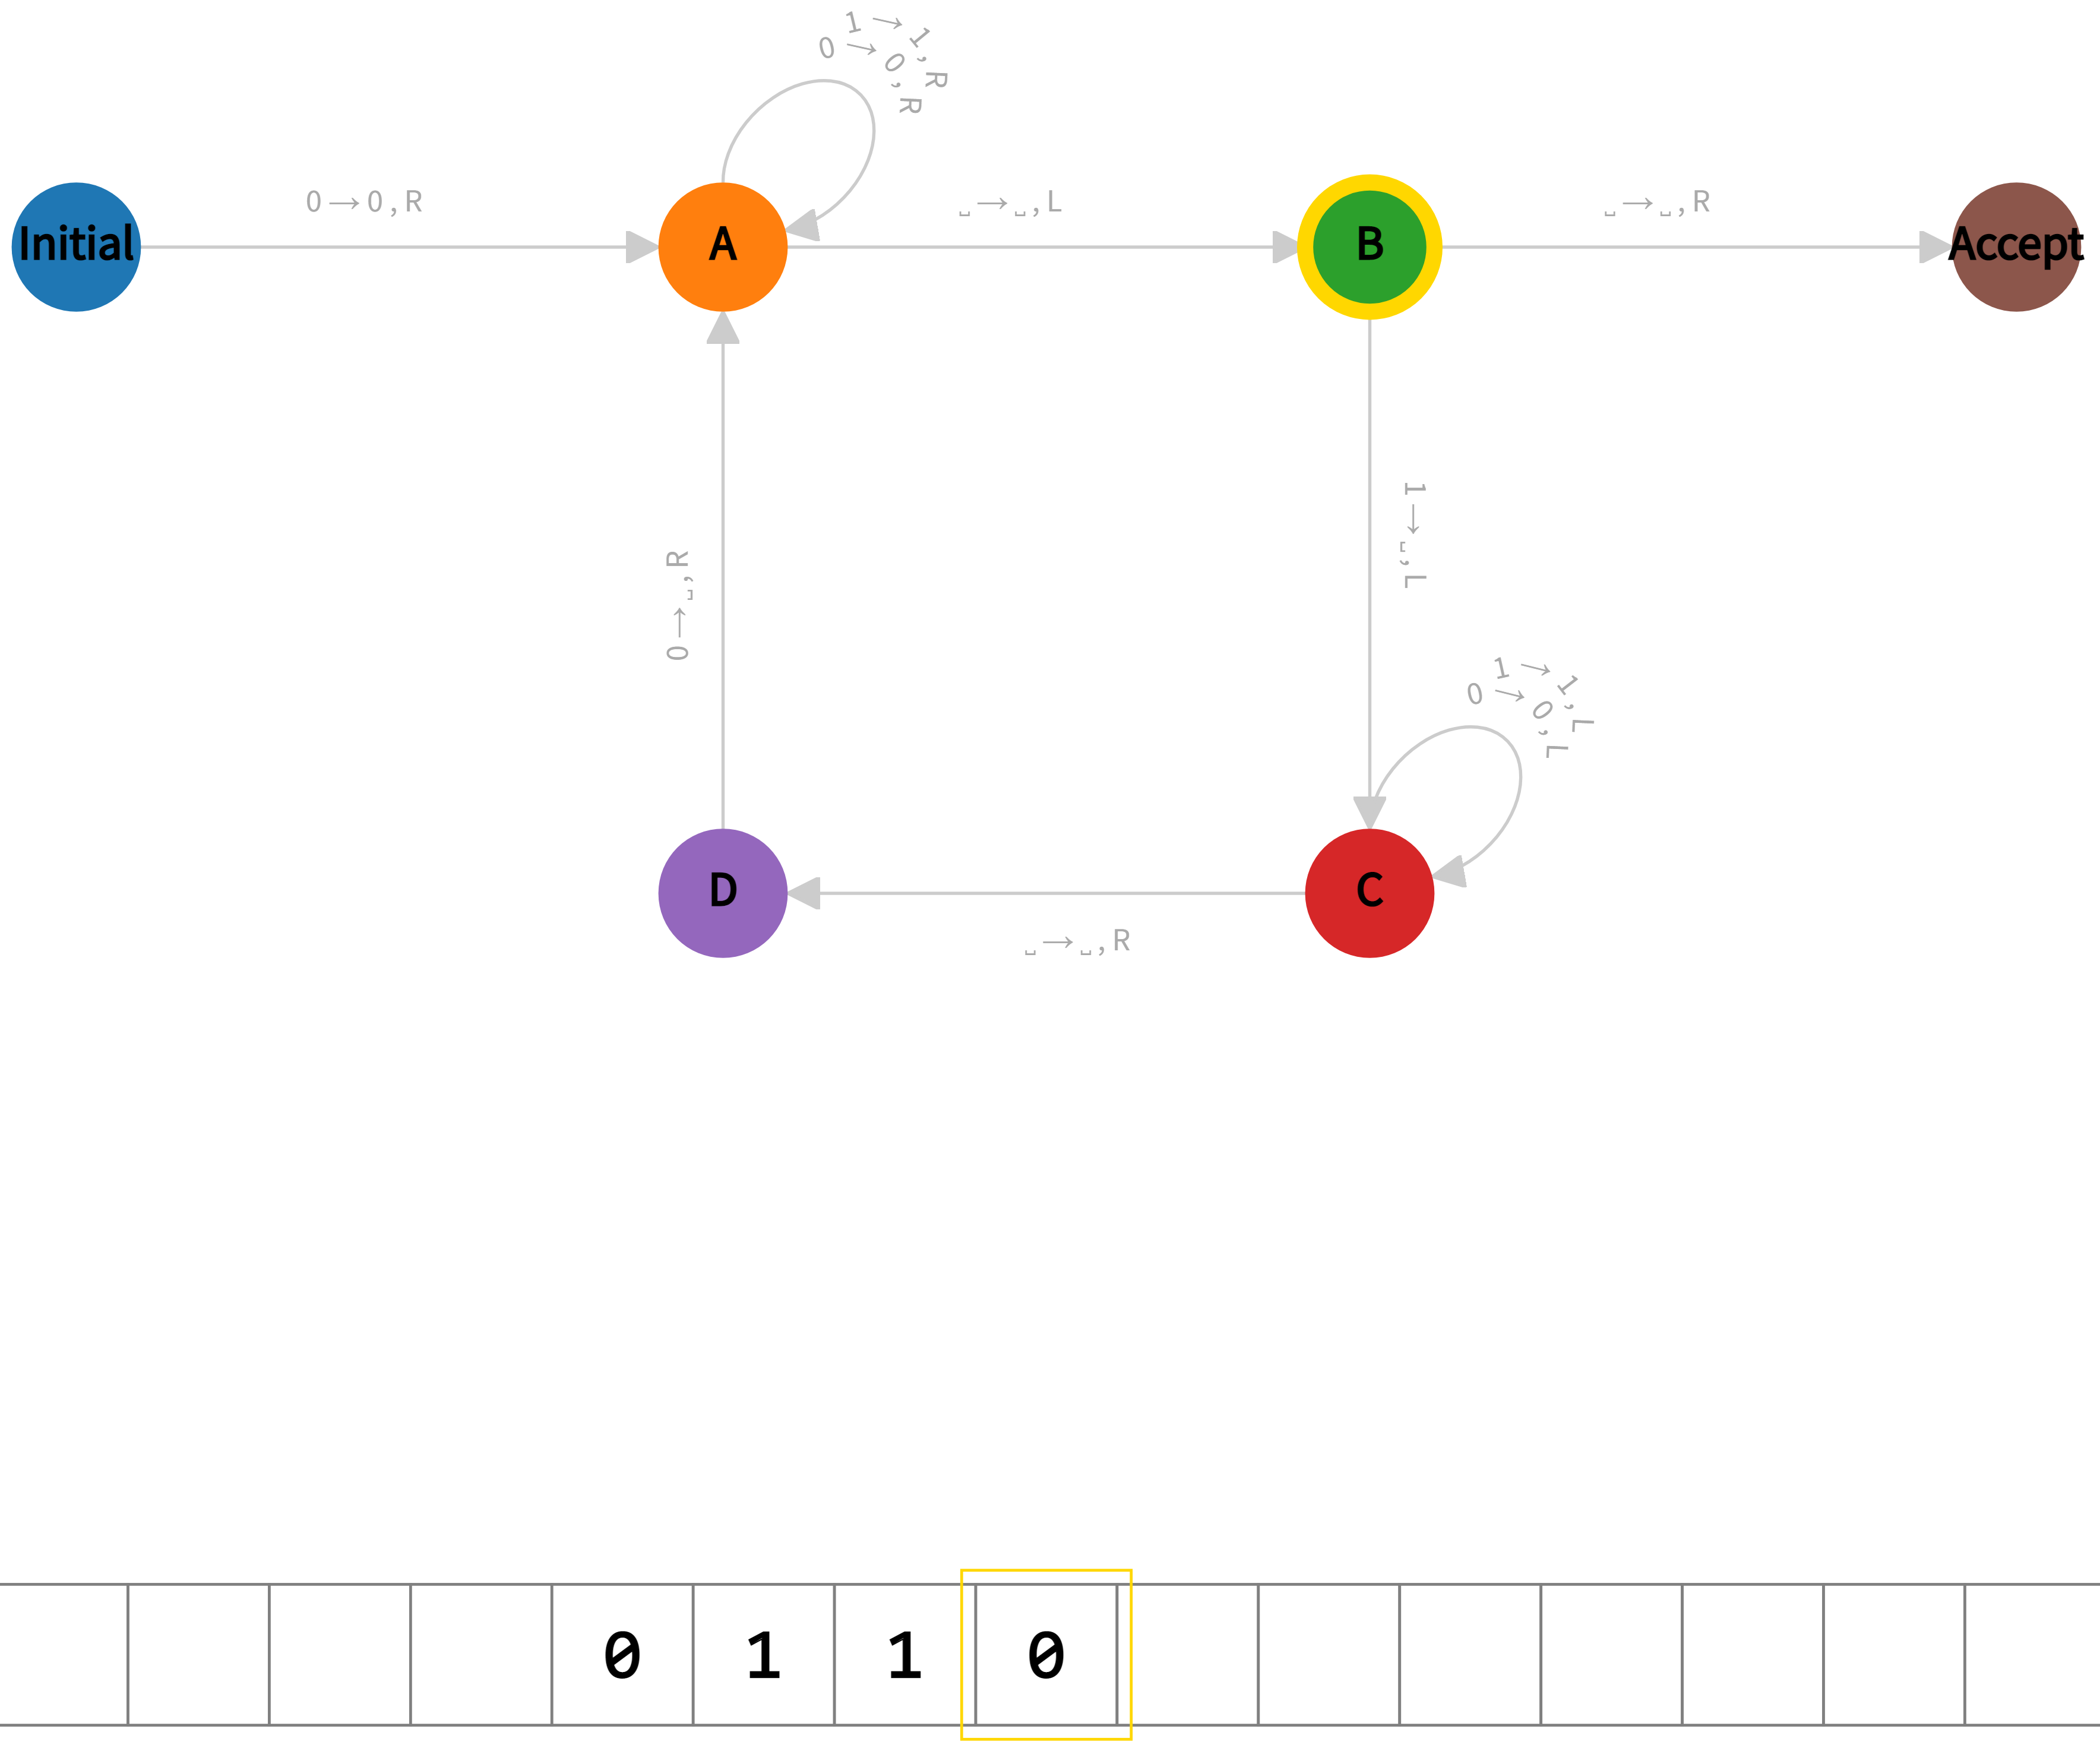
\includegraphics[width=\linewidth]{answers/img/q1-001101-end.png}
    \caption*{Figure (b): End State for $\mathbf{001101}$}
    \label{fig:001101-end}
  \end{minipage}
  \caption{States for $\mathbf{001101}$}
  \label{fig:in-001101}
\end{figure}

\subsubsection*{Input: 100011 $|$ Reject}
\label{q1-100011}

\begin{figure}[ht]
  \centering
  \begin{minipage}{.49\linewidth}
    \centering
    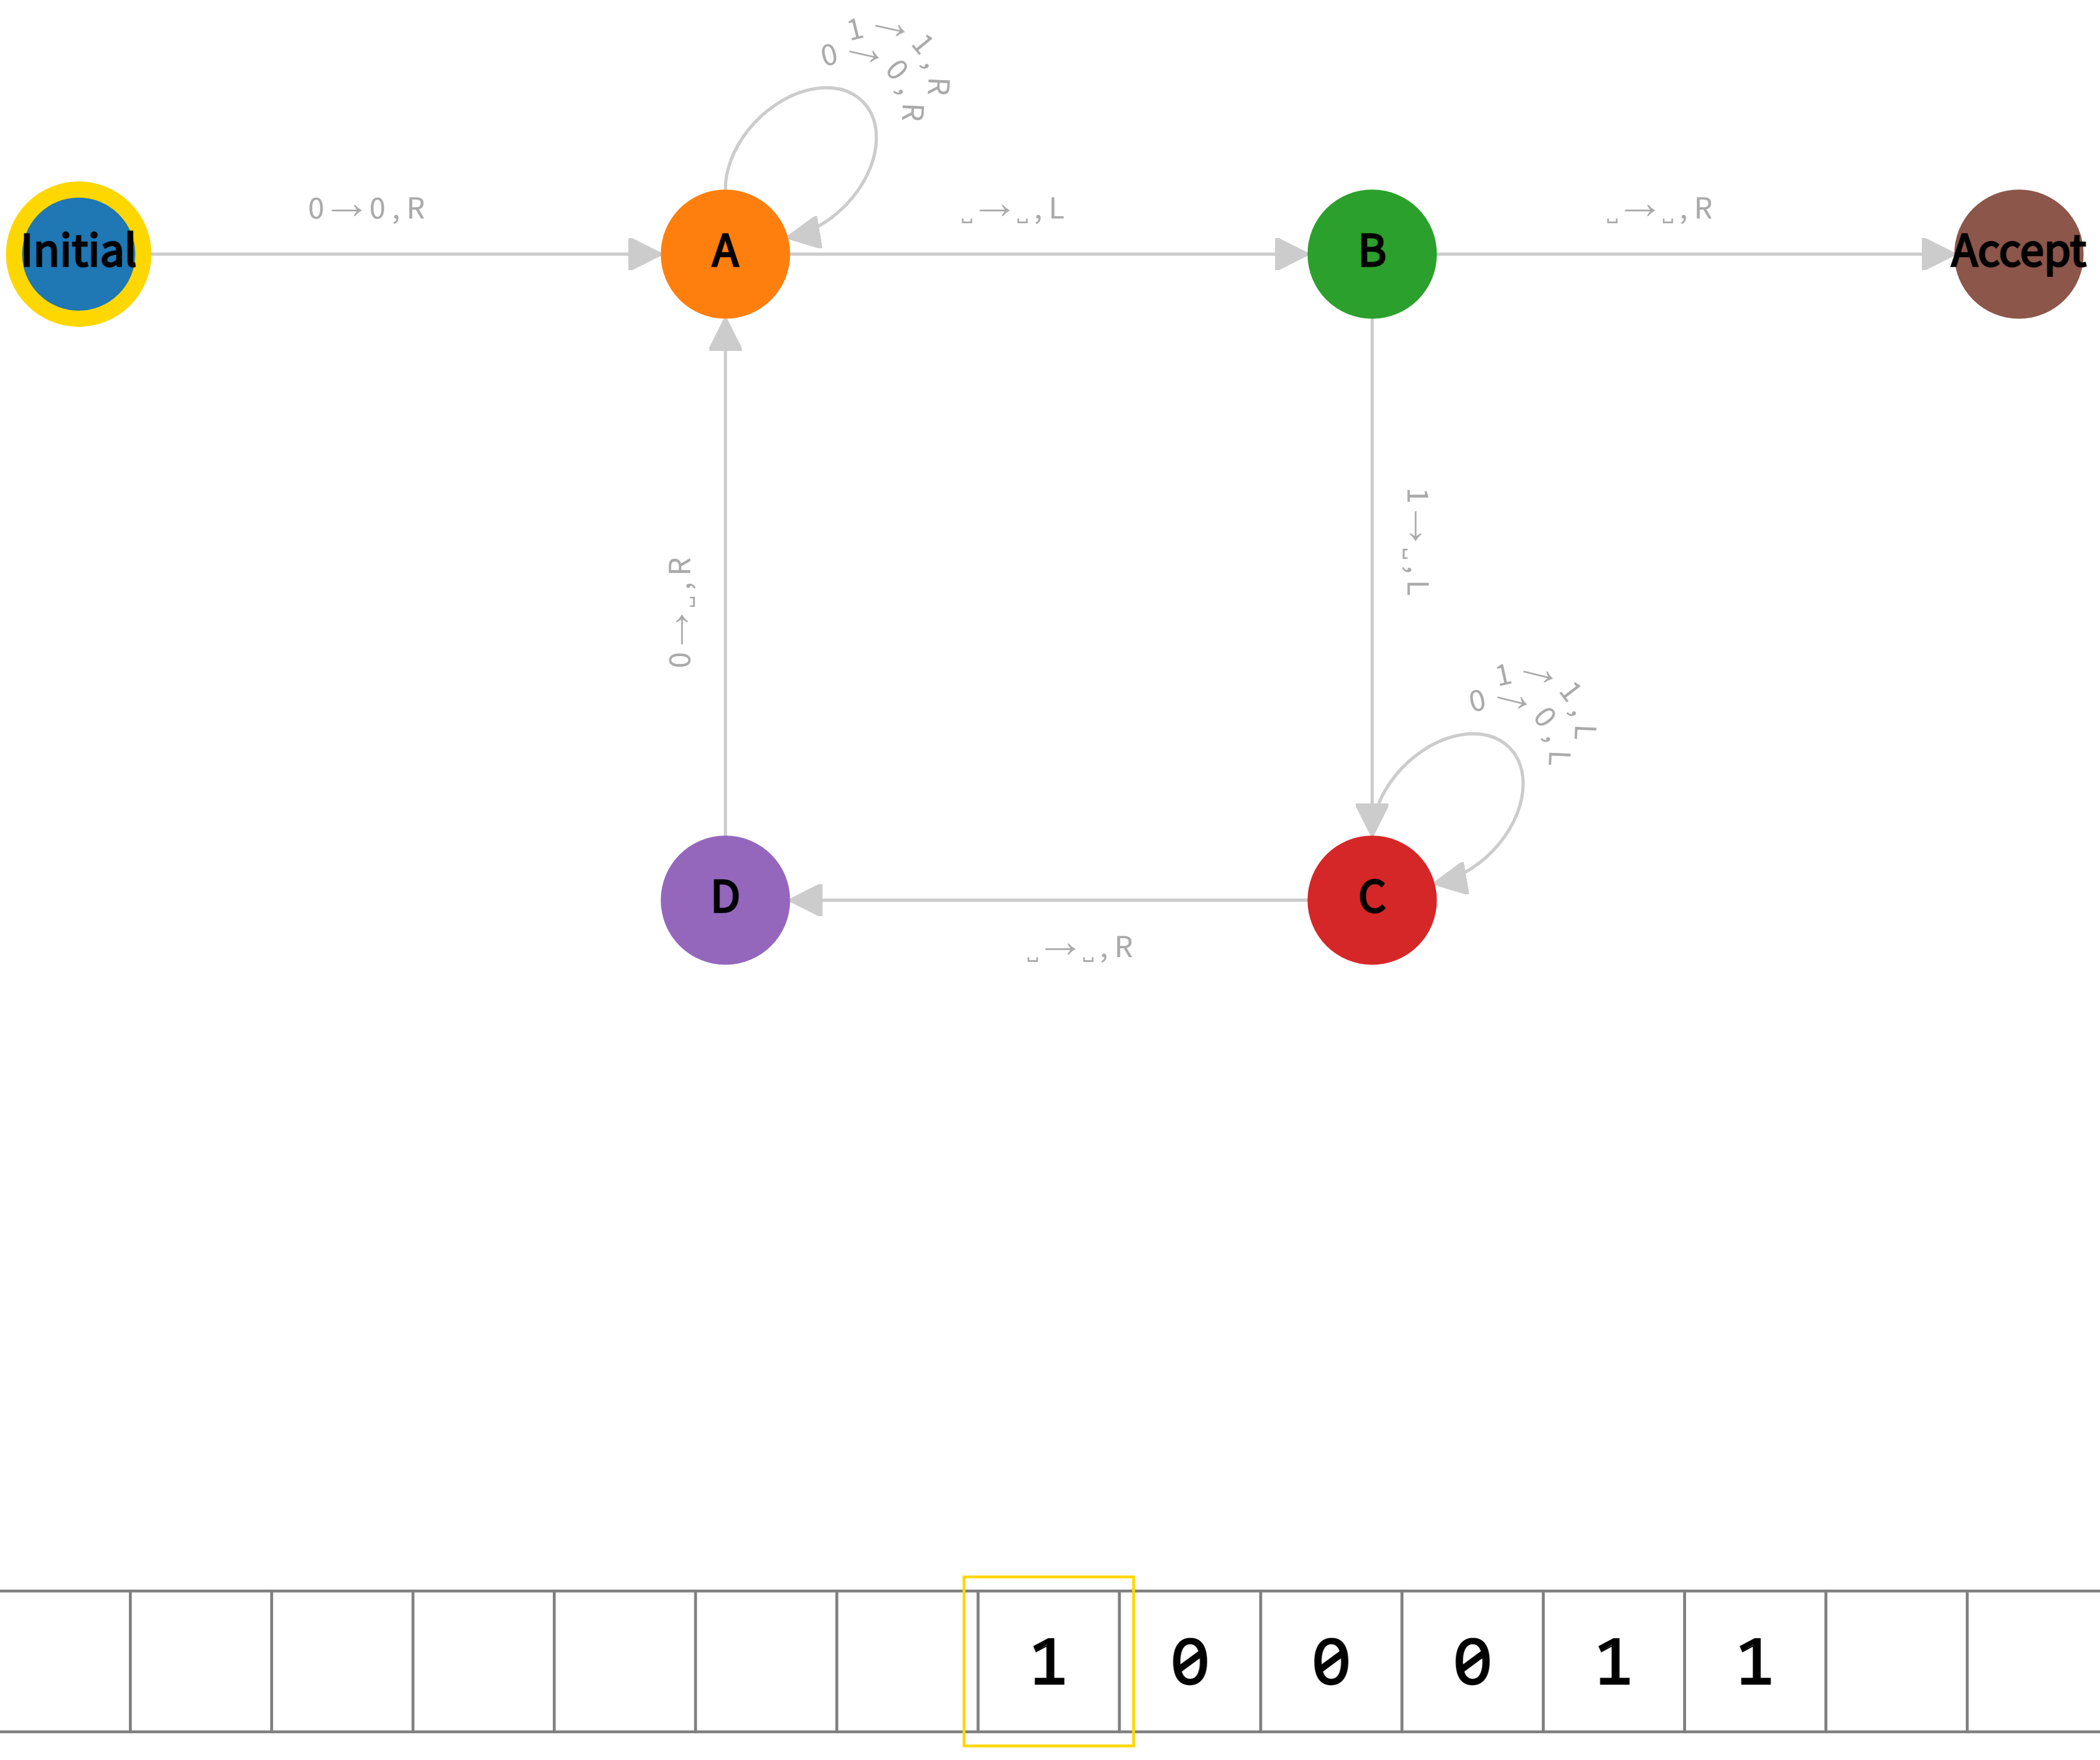
\includegraphics[width=\linewidth]{answers/img/q1-100011-initial.png}
    \caption*{Figure (a): Initial State for $\mathbf{100011}$}
    \label{fig:100011-initial}
  \end{minipage}
  \begin{minipage}{.49\linewidth}
    \centering
    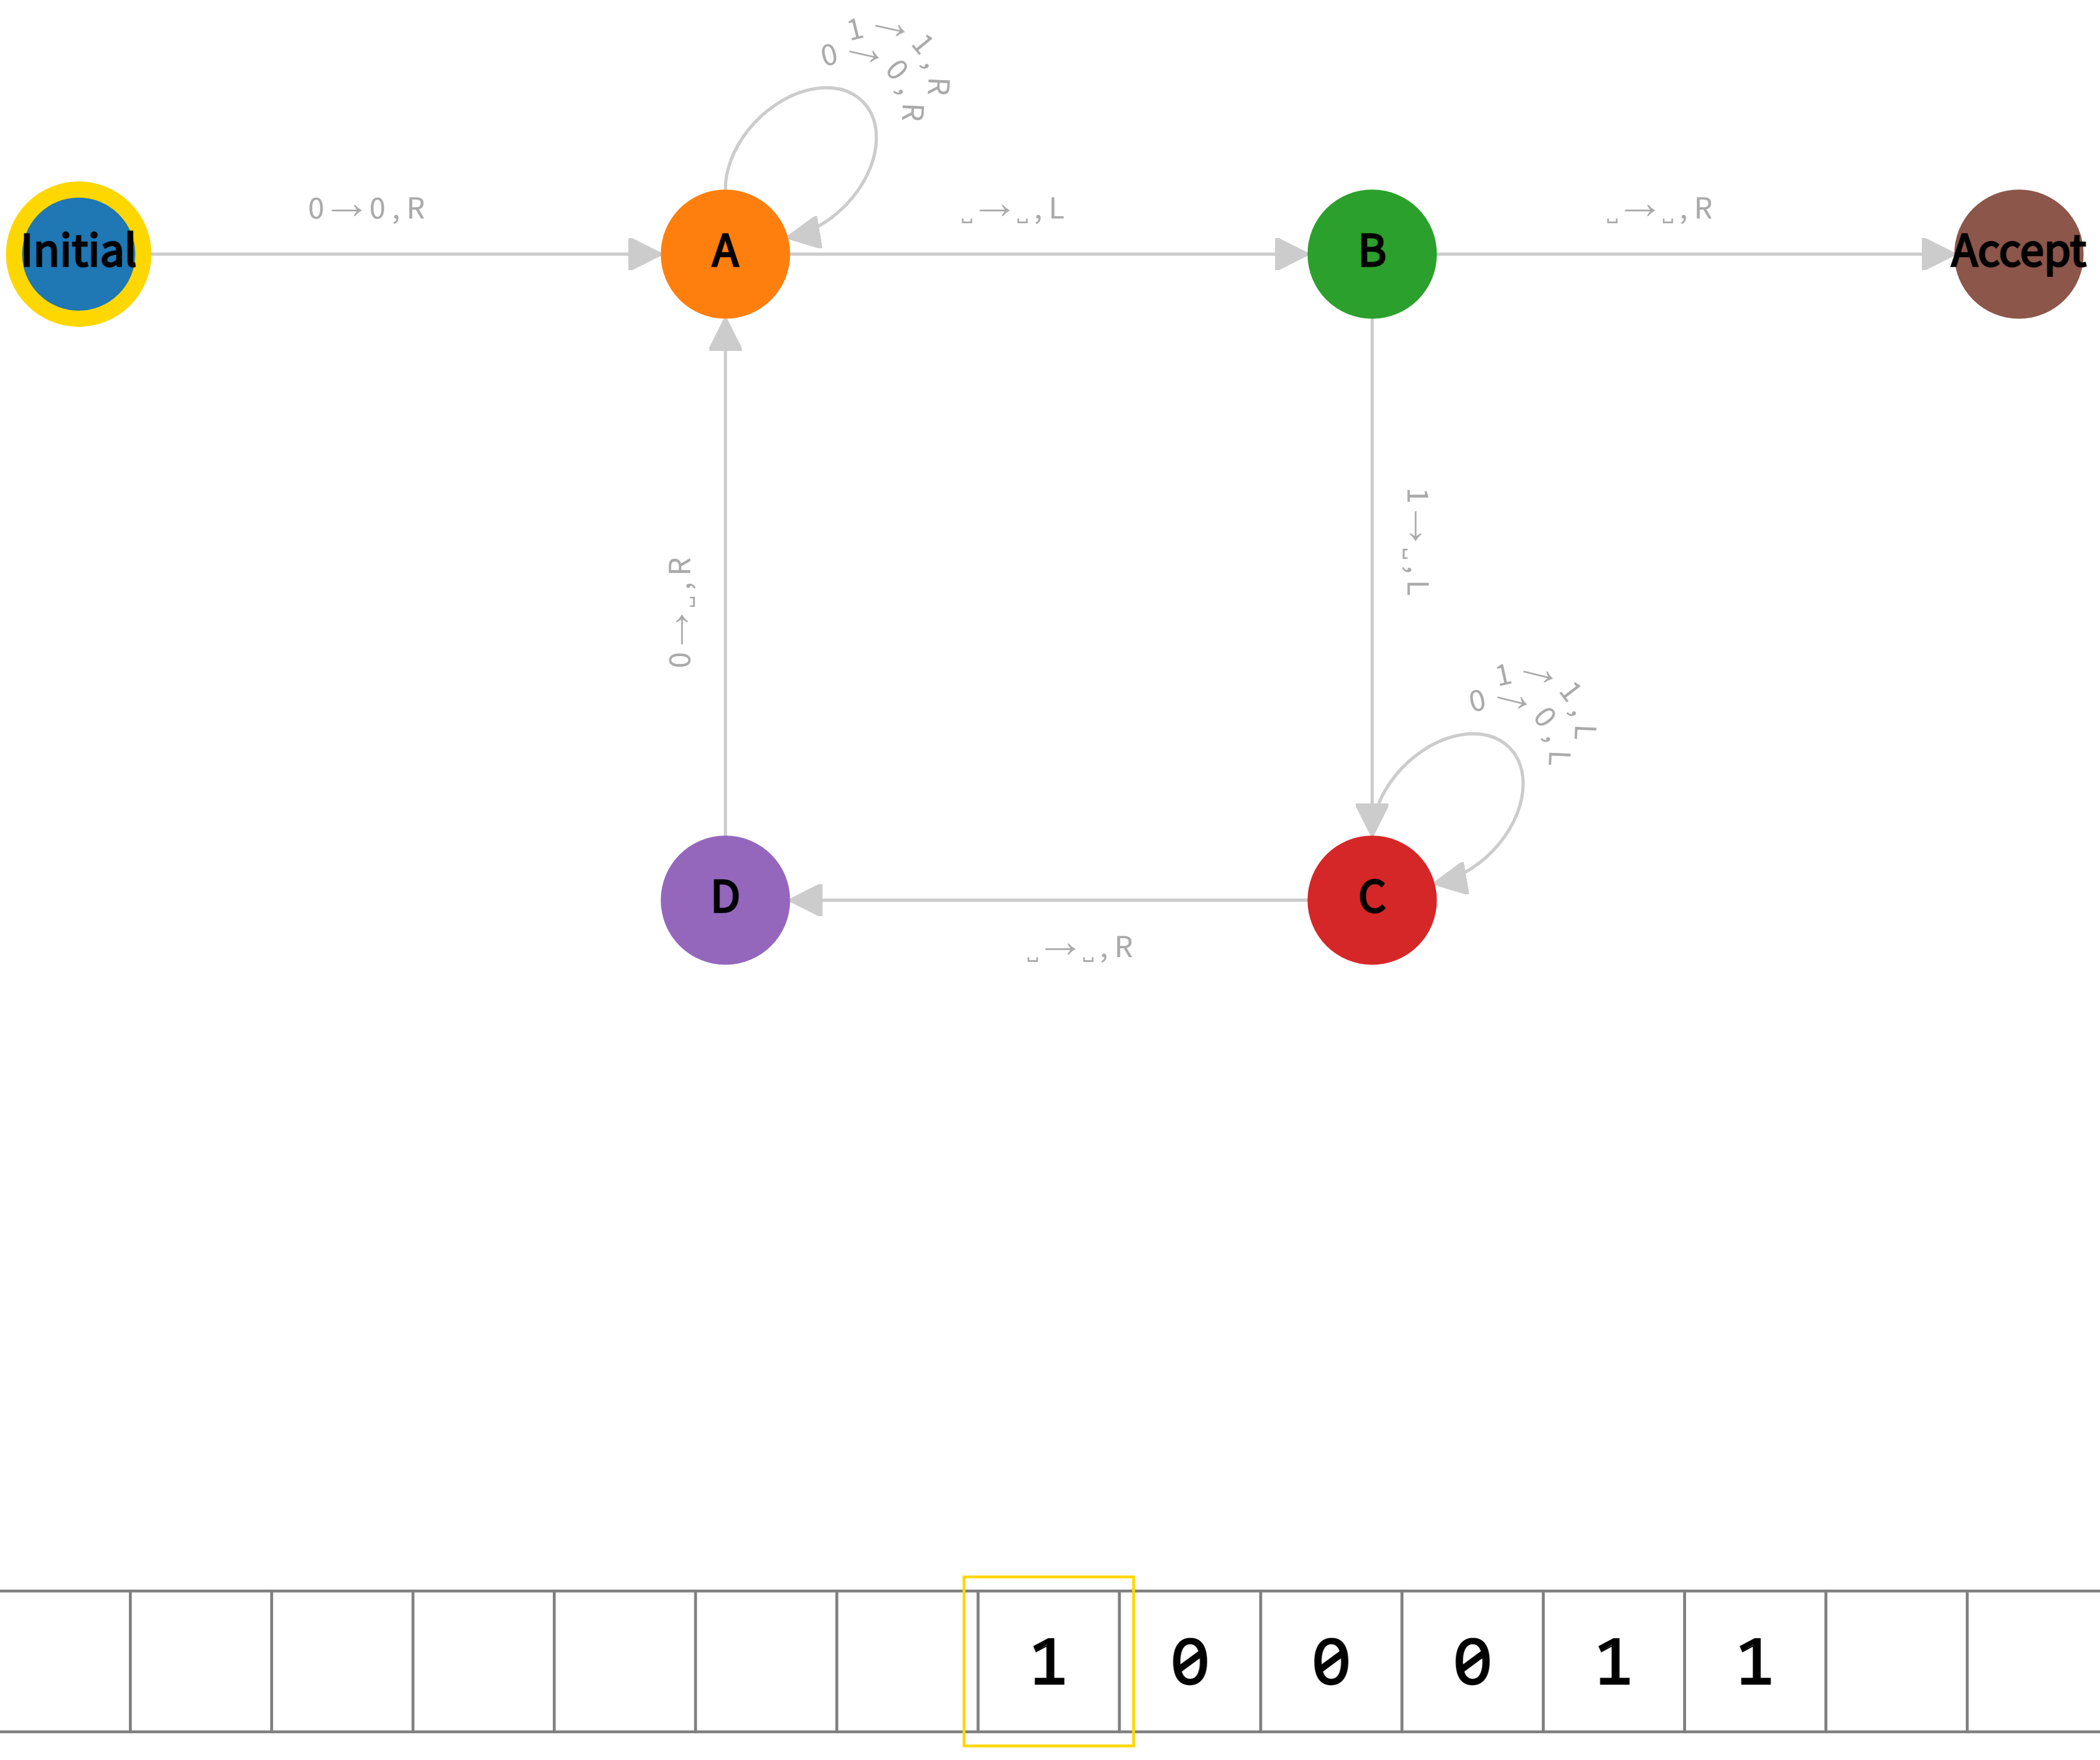
\includegraphics[width=\linewidth]{answers/img/q1-100011-end.png}
    \caption*{Figure (b): End State for $\mathbf{100011}$}
    \label{fig:100011-end}
  \end{minipage}
  \caption{States for $\mathbf{100011}$}
  \label{fig:in-100011}
\end{figure}

\vspace*{\fill}



% --- General Description ---

% Machine will start in the beginning of the string (namely, $0^{th}$ index). Then it will scan to the right for an $\blank$ symbol. 

% When it found the $\blank$ symbol, it will move to the left. 

% If there is a 1, then a $\blank$ will be written and start scanning to the left for another $blank$ symbol.

% If there is a $\blank$, then accepts

% When it found the first $blank$, it will move the right. If there is a 0, then a $\blank$ will be written.
